%\documentstyle[art10,titlepage,makeidx,twoside,EPSF/epsf,mytabbing]{j-article}

% euslisp
\newif\ifeuslisp
\euslisptrue

%%% added 2004.12.14
\documentclass[]{jarticle}
\usepackage{makeidx,mytabbing,fancyheadings}


\usepackage[dvipdfm]{graphicx,color,epsfig}
\let\epsfile=\epsfig
\usepackage[dvipdfm,bookmarks=true,bookmarksnumbered=true,bookmarkstype=toc]{hyperref}
\ifnum 42146=\euc"A4A2 \AtBeginDvi{\special{pdf:tounicode EUC-UCS2}}\else
\AtBeginDvi{\special{pdf:tounicode 90ms-RKSJ-UCS2}}\fi

%%%
\newcommand{\eusversion}{9.00}
\newcommand{\irteusversion}{1.00}


\flushbottom
\makeindex
\pagestyle{myheadings}
\oddsidemargin=0cm
\evensidemargin=0cm

% A4 size
\textwidth=16.5cm
\textheight=24.6cm
\topmargin=-0.8cm
\oddsidemargin= 0.5cm
\evensidemargin=0.5cm

% Letter size
%\topmargin=0.5cm
%\textwidth=17.6cm
%\textheight=23cm
%\oddsidemargin= 0.2cm
%\evensidemargin=0.2cm

\parindent=10pt
\parskip=1mm
%\baselineskip 14pt

\setcounter{totalnumber}{3}
\renewcommand{\topfraction}{0.99}       % 85% of a page (from page
                                        % top)
                                        % can be occupied by tbl / fig
                                        %
\renewcommand{\bottomfraction}{0.99}    % 85% of a page (from page
                                        % bottom)
                                        % can be occupied by tbl / fig
\renewcommand{\textfraction}{0.0}      % text shoud occupy 15% or
                                        % more in
                                        % a page
%\renewcommand{\floatpagefraction}{0.99} % 70% or more shoud occupy in
                                        % a
                                        % a float page


%%% removed 2004.12.14 \jintercharskip=0pt plus3.0pt minus1pt%

\usepackage{amsmath,amssymb}
\usepackage{cases} %% subnumcases
\newcommand{\labfig}[1]{\label{fig:#1}}
\newcommand{\labtab}[1]{\label{tab:#1}}
\newcommand{\labeq}[1]{\label{eq:#1}}
\newcommand{\labsec}[1]{\label{sec:#1}}
\newcommand{\labchap}[1]{\label{chap:#1}}
\newcommand{\labitem}[1]{\label{item:#1}}
\newcommand{\figlab}[1]{\labfig{#1}} % alias
\newcommand{\tablab}[1]{\labtab{#1}} % alias
\newcommand{\eqlab}[1]{\labeq{#1}} % alias
\newcommand{\eqlabel}[1]{\labeq{#1}} % alias
\newcommand{\equlab}[1]{\labeq{#1}} % alias
\newcommand{\reffig}[1]{{Fig.\ref{fig:#1}}~}
\newcommand{\reftab}[1]{{Table~\ref{tab:#1}}~}
\newcommand{\refeq}[1]{{Equation~\ref{eq:#1}}~}
\newcommand{\refchap}[1]{第\ref{chap:#1}章}
\newcommand{\refitem}[1]{\ref{item:#1}}
\newcommand{\refsec}[1]{第\ref{seq:#1}節}
\newcommand{\figref}[1]{\reffig{#1}} % alias
\newcommand{\tabref}[1]{\reftab{#1}} % alias
\renewcommand{\eqref}[1]{\refeq{#1}} % alias
\newcommand{\chapref}[1]{\refchap{#1}} % alias
\newcommand{\secref}[1]{\refsec{#1}} % alias
\newcommand{\bm}[1]{\mbox{\boldmath{$#1$}}}
\makeatletter
\newcommand{\footnoteref}[1]{\protected@xdef\@thefnmark{\ref{#1}}\@footnotemark}
\makeatother



\begin{document}

\newcommand{\ptext}[1]
{\tt \begin{quote} \begin{tabbing} #1 \end{tabbing} \end{quote} \rm}

\newcommand{\desclist}[1]{
\begin{list}{ }{\setlength{\rightmargin}{0mm}\topsep=0mm\partopsep=0mm}
\item #1
\end{list}
\vspace{3mm}}

\newcommand{\functiondescription}[4]{
\index{#1}
{\bf #1} \em #2 \rm \hfill [#3] 
%\if#4 \vspace{3mm} \\ \else \desclist{#4} \fi
%\ifx#4 \vspace{3mm} \\ \else \desclist{#4} \fi
 \desclist{\hspace{0mm}#4}
}

\newcommand{\bfx}[1]{\index{#1}{\bf #1}}
\newcommand{\emx}[1]{\index{#1}{\em #1}}

\newcommand{\longdescription}[3]{
\index{#1}
\begin{emtabbing}
{\bf #1} 
\it #2
\rm
\end{emtabbing}
\desclist{#3}
}

\newcommand{\funcdesc}[3]{\functiondescription{#1}{#2}{関数}{#3}}
\newcommand{\macrodesc}[3]{\functiondescription{#1}{#2}{マクロ}{#3}}
\newcommand{\specialdesc}[3]{\functiondescription{#1}{#2}{特殊}{#3}}
\newcommand{\methoddesc}[3]{\functiondescription{#1}{#2}{メソッド}{#3}}
\newcommand{\vardesc}[2]{\functiondescription{#1}{}{変数}{#2}}

\newcommand{\fundesc}[2]{\functiondescription{#1}{#2}{関数}{\hspace{0mm}}}
\newcommand{\macdesc}[2]{\functiondescription{#1}{#2}{マクロ}{\hspace{0mm}}}
\newcommand{\spedesc}[2]{\functiondescription{#1}{#2}{特殊}{\hspace{0mm}}}
\newcommand{\metdesc}[2]{\functiondescription{#1}{#2}{メソッド}{\hspace{0mm}}}

\newcommand{\constdesc}[2]{\functiondescription{#1}{}{定数}{#2}}

\newcommand{\classdesc}[4]{	%class, super slots description
\vspace{2mm} 
\index{#1}
{\Large {\bf #1 }} \hfill [クラス]  %super
\begin{tabbing}
\hspace{30mm} :super \hspace{5mm} \= {\bf #2} \\
\hspace{30mm} :slots \> #3 
\end{tabbing}
\vspace{4mm}
\desclist{#4}}

\newenvironment{refdesc}{
 \vspace{5mm} \parindent=0mm \topsep=0mm \parskip=0mm \leftmargin=10mm}{
             \parindent=10mm \topsep=3mm \parskip=1mm \leftmargin=0mm }


\date{}
\title{{\Huge \bf EusLisp} \\
{\large \bf EusLisp version \eusversion / irteus version \irteusversion} \\
{\LARGE \bf リファレンスマニュアル} \\
{\large -ロボットモデリングの拡張-} \\
\vspace{10mm}
%ETL-RM-87-06E \\
{\large ETL-TR-95-19 + JSK-TR-10-03} \\
{\large \today} \\ }

\author{
irteus \irteusversion\\
東京大学大学院 \\
情報理工学系研究科 知能機械情報学専攻\\
{\large 野沢 峻一 , 植田 亮平, 岡田 慧} \\
ueda@jsk.t.u-tokyo.ac.jp nozawa@jsk.t.u-tokyo.ac.jp k-okada@jsk.t.u-tokyo.ac.jp\\
〒113-8656 東京都文京区本郷7-3-1 工学部2号館7階73B2 
\\
EusLisp \eusversion\\
通商産業省 工業技術院 \\
電子技術総合研究所 知能システム部 \\
{\large 松井 俊浩, 原 功, 中垣 博文(九州電力)} \\
matsui@etl.go.jp, hara@etl.go.jp, nakagaki@etl.go.jp\\
〒305 茨城県つくば市梅園1-1-4 \\
}

\thispagestyle{empty}
\maketitle
\pagenumbering{roman}
\tableofcontents
% \listoffigures
% \listoftables
\bibliographystyle{plain}
\newpage
\pagenumbering{arabic}

\ifeuslisp
\part{EusLisp 基本}
\markboth{EusLisp version \eusversion リファレンスマニュアル (Part I)}{はじめに}
\input{jintro}
\input{jgenerals}
\input{jcontrols}
\input{jobjects}
%\input{predicates}
\input{jarith}
\input{jsymbols}
\input{jsequences}
\input{jio}
\input{jevaluation}
\newpage
\part{EusLisp 拡張}
\markboth{EusLisp version \eusversion リファレンスマニュアル (Part II)}{システム関数}
\input{jsysfunc}
\input{jvxw}
\input{jmthread}
\input{jmatrix}
\input{jgeometry}
\input{jcontact}
\input{jvoronoi}
\input{jgraphics}
\input{jxwindow}
\input{jxtoolkit}
\fi
%

\part{irteus 拡張}
\markboth{EusLisp version \eusversion リファレンスマニュアル (Part  III)}{ロボットモデリング関数}

\section{ロボットモデリング}

\subsection{ロボットのデータ構造とモデリング}

\subsubsection{ロボットのデータ構造と順運動学}

ロボットの構造はリンクと関節から構成されていると考えることが出来るが,
ロボットを関節とリンクに分割する方法として
\begin{itemize}
\item (a)切り離されるリンクの側に関節を含める
\item (b)胴体,あるいは胴体に近いほうに関節を含める
\end{itemize}
が考えられる.コンピュータのデータ構造を考慮し,
(a)が利用されている.その理由は胴体以外のすべてのリンクにおいて,
必ず関節を一つ含んだ構造となり,すべてのリンクを同一のアルゴリズムで扱う
ことが出きるためである.

この様に分割されたリンクを計算機上で表現するためにはツリー構造を利用する
ことが出来る.一般的にはツリー構造を作るときに二分木にすることでデータ構
造を簡略化することが多い.

ロボットのリンクにおける同次変換行列の求め方としては,関節回転座標系上に
原点をもつ$\Sigma_j$を設定し,親リンク座標系からみた回転軸ベクトルが
$a_j$, $\Sigma_j$の原点が$b_j$であり,回転の関節角度を$q_j$とする.

このとき$\Sigma_j$の親リンク相対の同次変換行列は
\[
 {}^iT_j =
 \left[
 \begin{array}{cc}
  e^{\hat{a}_jq_j} & b_j \\
  0~0~0 & 1
 \end{array}
 \right]
\]
と書くことが出来る.

ここで,$e^{\hat{a}_jq_j}$は,一定速度の角速度ベクトルによって生ずる回
転行列を与える以下のRodriguesの式を用いている.これを回転軸$a$周りに
$wt[rad]$だけ回転する回転行列を与えるものとして利用している.
\[
 e^{\hat{\omega}t} = E + \hat{a} sin (wt) + \hat{a}^2 (1 - cos(wt))
\]

親リンクの位置姿勢$p_i, R_i$が既知だとすると,$\Sigma_i$の同次変換行列を
\[
 T_i =
 \left[
 \begin{array}{cc}
  R_i & p_i \\
  0~0~0 & 1
 \end{array}
 \right]
\]
と作ることができ,ここから
\[
 T_j = T_i ~ {}^iT_j
\]
として計算できる.これをロボットのルートリンクから初めてすべてのリンクに
順次適用することでロボットの全身の関節角度情報から姿勢情報を算出すること
ができ,これを順運動学と呼ぶ.

\subsubsection{EusLispによる幾何情報のモデリング}

Euslispの幾何モデリングでは,基本モデル(body)の生成,bodyの合成関数,複
合モデル(bodyset)の生成と3つの段階がある.

これまでに以下のような基本モデルの生成,合成が可能な事を見てきている.
{\baselineskip=10pt
\begin{verbatim}
(setq c1 (make-cube 100 100 100))
(send c1 :locate #f(0 0 50))
(send c1 :rotate (deg2rad 30) :x)
(send c1 :set-color :yellow)
(objects (list c1))

(setq c2 (make-cylinder 50 100))
(send c2 :move-to
      (make-coords
       :pos #f(20 30 40)
       :rpy (float-vector 0 0 (deg2rad 90)))
      :world)
(send c2 :set-color :green)
(objects (list c1 c2))

(setq c3 (body+ c1 c2))
(setq c4 (body- c1 c2))
(setq c5 (body* c1 c2))
\end{verbatim}
}

bodysetはirteusで導入された複合モデルであり,bodyで扱えない複数の物体や
複数の色を扱うためのものである.

{\baselineskip=10pt
\begin{verbatim}
(setq c1 (make-cube 100 100 100))
(send c1 :set-color :red)
(setq c2 (make-cylinder 30 100))
(send c2 :set-color :green)
(send c1 :assoc c2)           ;;; これを忘れいように
(setq b1 (instance bodyset :init
                   (make-cascoords)
                   :bodies (list c1 c2)))
(objects (list b1))
\end{verbatim}
}

\subsubsection{幾何情報の親子関係を利用したサンプルプログラム}

{\baselineskip=10pt
\begin{verbatim}
(setq c1 (make-cube 100 100 100))
(setq c2 (make-cube 50 50 50))
(send c1 :set-color :red)
(send c2 :set-color :blue)
(send c2 :locate #f(300 0 0))
(send c1 :assoc c2)
(objects (list c1 c2))
(do-until-key
 (send c1 :rotate (deg2rad 5) :z)
 (send *irtviewer* :draw-objects)
 (x::window-main-one) ;; process window event
 )
\end{verbatim}
}

\subsubsection{bodyset-linkとjointを用いたロボット(多リンク系)のモデリング}

irteusではロボットリンクを記述するクラスとしてbodyset-link(irtmodel.l)
というクラスが用意されている.これは機構情報と幾何情報をもち,一般的な木
構造でロボットの構造が表現されている.また,jointクラスを用いて関節情報
を扱っている.

{\baselineskip=10pt
\begin{verbatim}
(defclass bodyset-link
  :super bodyset
  :slots (joint parent-link child-links analysis-level default-coords
                weight acentroid inertia-tensor
                angular-velocity angular-acceleration
                spacial-velocity spacial-acceleration
                momentum-velocity angular-momentum-velocity
                momentum angular-momentum
                force moment ext-force ext-moment))
\end{verbatim}
}

ジョイント(関節)のモデリングはjointクラス(irtmodel.l)を用いる.jointクラスは基底ク
ラスであり,実際にはrotational-joint, linear-joint等を利用する.
jointの子クラスで作られた関節は,:joint-angleメソッドで関節角度を指定す
ることが出来る.

{\baselineskip=10pt
\begin{verbatim}
(defclass joint
  :super propertied-object
  :slots (parent-link child-link joint-angle min-angle max-angle
	default-coords))
(defmethod joint
  (:init (&key name
               ((:child-link clink)) ((:parent-link plink))
               (min -90) (max 90) &allow-other-keys)
         (send self :name name)
         (setq parent-link plink child-link clink
               min-angle min max-angle max)
         self))

(defclass rotational-joint
  :super joint
  :slots (axis))
(defmethod rotational-joint
  (:init (&rest args &key ((:axis ax) :z) &allow-other-keys)
         (setq axis ax joint-angle 0.0)
         (send-super* :init args)
         self)
  (:joint-angle
   (&optional v)
   (when v
        (setq relang (- v joint-angle) joint-angle v)
        (send child-link :rotate (deg2rad relang) axis)))
     joint-angle))
\end{verbatim}
}

ここでは,joint, parent-link, child-links, defualt-coordsを利用する.

簡単な1関節ロボットの例としてサーボモジュールを作ってみると
{\baselineskip=10pt
\begin{verbatim}
(defun make-servo nil
  (let (b1 b2)
    (setq b1 (make-cube 35 20 46))
    (send b1 :locate #f(9.5 0 0))
    (setq b2 (make-cylinder 3 60))
    (send b2 :locate #f(0 0 -30))
    (setq b1 (body+ b1 b2))
    (send b1 :set-color :gray20)
    b1))

(defun make-hinji nil
  (let ((b2 (make-cube 22 16 58))
        (b1 (make-cube 26 20 54)))
    (send b2 :locate #f(-4 0 0))
    (setq b2 (body- b2 b1))
    (send b1 :set-color :gray80)
    b2))

(setq h1 (instance bodyset-link :init (make-cascoords) :bodies (list (make-hinji))))
(setq s1 (instance bodyset-link :init (make-cascoords) :bodies (list (make-servo))))
(setq j1 (instance rotational-joint :init :parent-link h1 :child-link s1 :axis :z))
;; instance cascaded coords
(setq r (instance cascaded-link :init))
(send r :assoc h1)
(send h1 :assoc s1)
(setq (r . links) (list h1 s1))
(setq (r . joint-list) (list j1))
(send r :init-ending)
\end{verbatim}
}

となる.

ここでは,\verb|h1|,\verb|s1|という\verb|bodyset-link|と,
\verb|j1|という\verb|rotational-joint|を作成し,ここから
\verb|cascaded-link|という,連結リンクからなるモデルを生成している.
\verb|cascaded-link|は\verb|cascaded-coords|の子クラスであるため,
\verb|r (cascaded-link)|,\verb|h1|,\verb|s1|の座標系の親子関係を
\verb|:assoc|を利用して設定している.

\verb|(r . links)|という記法は\verb|r|というオブジェクトのスロット変数
     (メンバ変数)である\verb|links|にアクセスしている.ここでは,
\verb|links|および\verb|joint-list|に適切な値をセットし,
\verb|(send r :init-ending)|として必要な初期設定を行っている.

これで\verb|r|という2つのリンクと1つの関節情報
を含んだ1つのオブジェクトを生成できる.これで例えば
\verb|(objects (list h1 s1))|ではなく,
\verb|(objects (list r))|としてロボットをビューワに表示できる.
また,\verb|(send r :locate #f(100 0 0))|などの利用も可能になっている.

\verb|cascaded-link|クラスのメソッドの利用例としては以下ある.
\verb|:joint-list|,\verb|:links|といった関節リストやリンクリストへの
アクセサに加え,関節角度ベクトルへのアクセスを提供する
\verb|:angle-vector|メソッドが重要である.これを引数なしで呼び出せば現
在の関節角度が得られ,これに関節角度ベクトルを引数に与えて呼び出せば,その引
数が示す関節角度ベクトルをロボットモデルに反映させることができる.
{\baselineskip=10pt
\begin{verbatim}
$ (objects (list r))
(#<servo-model #X628abb0  0.0 0.0 0.0 / 0.0 0.0 0.0>)
;; useful cascaded-link methods
$ (send r :joint-list)
(#<rotational-joint #X6062990 :joint101067152>)
$ (send r :links)
(#<bodyset-link #X62ccb10 :bodyset103598864  0.0 0.0 0.0 / 0.0 0.0 0.0>
 #<bodyset-link #X6305830 :bodyset103831600  0.0 0.0 0.0 / 0.524 0.0 0.0>)
$ (send r :angle-vector)
#f(0.0)
$ (send r :angle-vector (float-vector 30))
#f(30.0)
\end{verbatim}
}

\subsubsection{cascaded-linkを用いたロボット(多リンク系)のモデリング}

一方で多リンク系のモデリング用のクラスとしてcascaded-linkというクラス
がある.
これには,links, joint-listというスロット変数があり,ここにbodyset-link,
ならびにjointのインスタンスのリストをバインドして利用する.
以下は,
\verb|cascaded-link|の子クラスを定義しここでロボットモデリングに
関する初期化処理を行うという書き方の例である.


{\baselineskip=10pt
\begin{verbatim}
(defclass cascaded-link
  :super cascaded-coords
  :slots (links joint-list bodies collision-avoidance-links))

(defmethod cascaded-link
  (:init (&rest args &key name &allow-other-keys)
         (send-super-lexpr :init args)
         self)
  (:init-ending
   ()
   (setq bodies (flatten (send-all links :bodies)))
   (dolist (j joint-list)
     (send (send j :child-link) :add-joint j)
     (send (send j :child-link) :add-parent-link (send j :parent-link))
     (send (send j :parent-link) :add-child-links (send j :child-link)))
   (send self :update-descendants))
)
\end{verbatim}
}

{\baselineskip=10pt
\begin{verbatim}

(defclass servo-model
  :super cascaded-link
  :slots (h1 s1 j1))
(defmethod servo-model
  (:init ()
   (let ()
     (send-super :init)
     (setq h1 (instance bodyset-link :init (make-cascoords) :bodies (list (make-hinji))))
     (setq s1 (instance bodyset-link :init (make-cascoords) :bodies (list (make-servo))))

     (setq j1 (instance rotational-joint :init :parent-link h1 :child-link s1 :axis :z))

     ;; instance cascaded coords
     (setq links (list h1 s1))
     (setq joint-list (list j1))
     ;;
     (send self :assoc h1)
     (send h1 :assoc s1)
     ;;
     (send self :init-ending)
     self))
  ;;
  ;; (send r :j1 :joint-angle 30)
  (:j1 (&rest args) (forward-message-to j1 args))
  )

(setq r (instance servo-model :init))
\end{verbatim}
}

このようなクラスを定義して\verb|(setq r (instance servo-model :init))|
としても同じようにロボットモデルのインスタンスを作成することができ,先
ほどのメソッドを利用できる.クラス定義するメリットは
\verb|(:j1 (&rest args) (forward-message-to j1 args))|というメソッド定
義により,関節モデルのインスタンスへのアクセサを提供することができる.
これにより,特定の関節だけの値を知りたいとき,あるいは値をセットしたい
時には\verb|(send r :j1 :joint-angle)|や
\verb|(send r :j1 :joint-angle 30)|
という指示が可能になっている.
このロボットを動かす場合は前例と同じように

{\baselineskip=10pt
\begin{verbatim}
(objects (list r))
(dotimes (i 300)
  (send r :angle-vector (float-vector (* 90 (sin (/ i 100.0)))))
  (send *irtviewer* :draw-objects))
\end{verbatim}
}

などとするとよい.

{\baselineskip=10pt
\begin{verbatim}
(setq i 0)
(do-until-key
  (send r :angle-vector (float-vector (* 90 (sin (/ i 100.0)))))
  (send *irtviewer* :draw-objects)
  (incf i))
\end{verbatim}
}
とすると,次にキーボードを押下するまでプログラムは動きつづける.

さらに,少し拡張して
これを用いて3リンク2ジョイントのロボットをモデリングした例が以下にな
る.:joint-angleというメソッドに\#f(0 0)というベクトルを引数に与えるこ
とで全ての関節角度列を指定することが出来る.

{\baselineskip=10pt
\begin{verbatim}
(defclass hinji-servo-robot
  :super cascaded-link)
(defmethod hinji-servo-robot
  (:init
   ()
   (let (h1 s1 h2 s2 l1 l2 l3)
     (send-super :init)
     (setq h1 (make-hinji))
     (setq s1 (make-servo))
     (setq h2 (make-hinji))
     (setq s2 (make-servo))
     (send h2 :locate #f(42 0 0))
     (send s1 :assoc h2)
     (setq l1 (instance bodyset-link :init (make-cascoords) :bodies (list h1)))
     (setq l2 (instance bodyset-link :init (make-cascoords) :bodies (list s1 h2)))
     (setq l3 (instance bodyset-link :init (make-cascoords) :bodies (list s2)))
     (send l3 :locate #f(42 0 0))

     (send self :assoc l1)
     (send l1 :assoc l2)
     (send l2 :assoc l3)

     (setq joint-list
           (list
            (instance rotational-joint
                      :init :parent-link l1 :child-link l2
                      :axis :z)
            (instance rotational-joint
                      :init :parent-link l2 :child-link l3
                      :axis :z)))
     (setq links (list l1 l2 l3))
     (send self :init-ending)
     )))
(setq r (instance hinji-servo-robot :init))
(objects (list r))

(dotimes (i 10000)
  (send r :angle-vector (float-vector (* 90 (sin (/ i 500.0))) (* 90 (sin (/ i 1000.0)))))
  (send *irtviewer* :draw-objects))
\end{verbatim}
}

\subsubsection{EusLispにおける順運動学計算}

順運動学計算を行うには,cascaded-corods, bodyset, bodyset-link 各クラ
スに定義された :worldcoords メソッドを用いる.
:worldcoords メソッドは,ルートリンクが見つかる(親リンクがなくなる)
か, スロット変数 changed が nil であるリンク
(一度順運動学計算を行ったことがある)が見つかるまで
さかのぼって親リンクの :worldcoords メソッドを呼び出すことで
順運動学計算を行う.
その際,スロット変数 changed を nil で上書く.
したがって,二度目の :worldcoords メソッドの呼び出しでは,一度計算され
たリンクの順運動学計算は行われず,即座にリンクの位置姿勢情報を取り出す
ことができる.

また,bodyset-link クラスの :worldcoords メソッドは, level 引数を取る
ことができ,それが :coords である場合には,リンクのもつ bodies スロット変数
の順運動学計算は行われない.
bodies にリンクの頂点を構成する faceset が含まれている場合には,これら
についての順運動学計算を省略することで大幅な高速化が期待できるだろう.
なお, level 引数の初期値には,リンクのもつ analysis-level スロット変数
が用いられるため,常に bodies の順運動学計算を行わない場合は,
リンクのインスタンス l について
\verb|(send l :analysis-level :coords)|
とすればよい.

{\baselineskip=10pt
\begin{verbatim}
(defmethod bodyset-link
  (:worldcoords
   (&optional (level analysis-level))
   (case
    level
    (:coords (send-message self cascaded-coords :worldcoords))
    (t       (send-super :worldcoords)))
   ))

(defmethod bodyset
  (:worldcoords
   ()
   (when changed
     (send-super :worldcoords)
     (dolist (b bodies) (send b :worldcoords)))
   worldcoords))

(defmethod cascaded-coords
 (:worldcoords  ()      ;calculate rot and pos in the world
   (when changed
      (if parent
          (transform-coords (send parent :worldcoords) self
worldcoords)
          (send worldcoords :replace-coords self))
      (send self :update)
      (setf changed nil))
   worldcoords))
\end{verbatim}
}

\subsection{ロボットの動作生成}

%% \subsubsection{座標系の表現}
%% 特に断らない限り,添字のない物理量は絶対(世界)座標系で表したものとする.
%% 座標系$\Sigma_i$で表記した物理量は$^{i}p$のように左肩の添字で表現する.
%% 剛体の姿勢は直交行列で表し,座標系は右手系のみとする.

%% マ二ピュレータのエンドエフェクタの位置・姿勢は
%% 順運動学の式\eqref{forward-kinematics}によって与えられる.
%% \begin{eqnarray}
%%   ^0_n\bm{H}(\bm{\theta}) = ^0_1\bm{H}(\theta_1)^1_2\bm{H}(\theta_2)
%%   \dots ^{n-1}_n\bm{H}(\theta_n)
%%   \eqlabel{forward-kinematics}
%% \end{eqnarray}

%% ここで, $^i_j\bm{H}$は座標系$\Sigma_i$から見た座標系$\Sigma_j$の
%% 相対位置・姿勢を表現する$4\times4$の同次変換行列である.


\subsubsection{逆運動学}
逆運動学においては, エンドエフェクタの位置・姿勢$^0_n\bm{H}$から
マニピュレータの関節角度ベクトル
$\bm{\theta}=(\theta_1, \theta_2, ..., \theta_n)^T$
を求める.

%% 同次変換行列$^0_n\bm{H}$は6自由度を有するので, $n \geq 6$であるマニピュレータに
%% 対しては解が複数存在, もしくは存在しない場合がある.
%% もちろんここでは, 逆運動学の目標が6自由度全てについて, 拘束するとは限ら
%% ないことに留意する必要がある.

%% ??
ここで, %%ルートリンクからの
エンドエフェクタの%%相対
位置・姿勢$\bm{r}$
は関節角度ベクトルを用いて
\begin{eqnarray}
  \bm{r} = \bm{f}(\bm{\theta}) \eqlabel{forward-kinematics-functional}
\end{eqnarray}
とかける.
%%$\bm{r} = (x, y, z, \alpha, \beta, \gamma)^T$とすると
\eqref{forward-kinematics-functional}は\eqref{inverse-kinematics-func}
のように記述し,関節角度ベクトルを求める.
%%従って, 逆運動学を与える式は以下のように記述できる.
\begin{eqnarray}
  \bm{\theta} = \bm{f}^{-1}(\bm{r}) \eqlabel{inverse-kinematics-func}
\end{eqnarray}

\eqlabel{inverse-kinematics-func}における$f^{-1}$は一般に非線形な関数となる.
そこで\eqlabel{forward-kinematics-functional}を時刻tに関して微分することで,
線形な式
\begin{eqnarray}
 \dot{\bm{r}} &=& \frac{\partial \bm{f}}{\partial \bm{\theta}}
   (\bm{\theta})\dot{\bm{\theta}} \\
 &=& \bm{J}(\bm{\theta})\dot{\bm{\theta}}
 \eqlabel{inverse-kinematics-base}
\end{eqnarray}
を得る.
ここで, $\bm{J}(\bm{\theta})$は$m \times n$のヤコビ行列である.
$m$はベクトル$\bm{r}$の次元, $n$はベクトル$\bm{\theta}$の次元である.
$\bm{\dot{r}}$は速度・角速度ベクトルである.

ヤコビ行列が正則であるとき逆行列$\bm{J}(\bm{\theta})^{-1}$を用いて
以下のようにしてこの線型方程式の解を得ることができる.
\begin{eqnarray}
  \dot{\bm{\theta}} = \bm{J}(\bm{\theta})^{-1}\dot{\bm{r}}
  \eqlabel{inverse-kinematics}
\end{eqnarray}

しかし, 一般にヤコビ行列は正則でないので,
ヤコビ行列の疑似逆行列$\bm{J}^{\#}(\bm{\theta})$
が用いられる(\eqref{psuedo-inverse-matrix}).
\begin{eqnarray}
 \bm{A}^{\#} = \left\{
                \begin{array}{l l}
                 & \bm{A}^{-1} \ ( m = n = rank \bm{A}) \\
                 & \bm{A}^T \ (\bm{A}\bm{A}^T)^{-1} ( n > m = rank \bm{A}) \\
                 & (\bm{A}^T\bm{A})^{-1}\bm{A}^T \ ( m > n = rank \bm{A})
                \end{array}
	  \right.
 \eqlabel{psuedo-inverse-matrix}
\end{eqnarray}

\eqref{inverse-kinematics-base}は,
$m>n$のときは\eqref{inverse-kinematics-error-func}を,
$n>=m$のときは\eqref{inverse-kinematics-min-func}を,
最小化する最小二乗解を求める問題と捉え,解を得る.

\begin{eqnarray}
 \min_{\dot{\bm{\theta}}} \left(\dot{\bm{r}} - \bm{J}(\bm{\theta})\dot{\bm{\theta}}\right)^{T}
\left(\dot{\bm{r}} - \bm{J}(\bm{\theta})\dot{\bm{\theta}}\right)
 \eqlabel{inverse-kinematics-error-func}
\end{eqnarray}
\begin{eqnarray}
 \min_{\dot{\bm{\theta}}} & \dot{\bm{\theta}}^{T}\dot{\bm{\theta}}\\
\nonumber s.t. & \dot{\bm{r}} = \bm{J}(\bm{\theta})\dot{\bm{\theta}}
 \eqlabel{inverse-kinematics-min-func}
\end{eqnarray}

関節角速度は次のように求まる.
\begin{eqnarray}
 \dot{\bm{\theta}} = \bm{J}^{\#}(\bm{\theta})\dot{\bm{r}} + 
  \left(\bm{E}_n - \bm{J}^{\#}(\bm{\theta})\bm{J}(\bm{\theta})\right)\bm{z}
  \eqlabel{inverse-kinematics-lagrangian-formula}
\end{eqnarray}

しかしながら, \eqref{inverse-kinematics-lagrangian-formula}に従って解を
求めると, ヤコビ行列$\bm{J}(\bm{\theta})$がフルランクでなくなる特異点に近づく
と, $\left|\dot{\bm{\theta}}\right|$が大きくなり不安定な振舞いが生じる.
そこで, Nakamura et al.のSR-Inverse\footnote{
Inverse kinematic solutions with singularity robustness for robot
manipulator control: Y.Nakamura and H. Hanafusa, Journal of Dynamic Systems, Measurement, and Control,
vol. 108, pp 163-171, 1986
}
を用いること
で, この特異点を回避する.

本研究では
ヤコビ行列の疑似逆行列$\bm{J}^{\#}(\bm{\theta})$の代わりに,
\eqref{SR-inverse-jacobian}に示す$\bm{J}^{*}(\bm{\theta})$
を用いる.
\begin{eqnarray}
 \bm{J}^{*}(\bm{\theta})
  = \bm{J}^T\left(\bm{J}\bm{J}^T + \epsilon \bm{E}_m\right)^{-1}
 \eqlabel{SR-inverse-jacobian}
\end{eqnarray}

これは, \eqref{inverse-kinematics-error-func}の代わりに,
\eqref{SR-inverse-error-func}を最小化する最適化問題を
解くことにより得られたものである.
\begin{eqnarray}
 \min_{\dot{\bm{\theta}}}
\{
 \dot{\bm{\theta}}^T \dot{\bm{\theta}}
+
\epsilon
\left(\dot{\bm{r}} - \bm{J}(\bm{\theta})\dot{\bm{\theta}}\right)^T
\left(\dot{\bm{r}} - \bm{J}(\bm{\theta})\dot{\bm{\theta}}\right)
\}
 \eqlabel{SR-inverse-error-func}
\end{eqnarray}

ヤコビ行列$\bm{J}(\bm{\theta})$が特異点に近づいているかの指標には
可操作度$\kappa(\bm{\theta})$\footnote{
ロボットアームの可操作度, 吉川恒夫, 日本ロボット学会誌, vol. 2, no. 1,
pp. 63-67, 1984.
}
が用いられる(\eqref{manipulability}).
\begin{eqnarray}
 \kappa(\bm{\theta}) = \sqrt{\bm{J}(\bm{\theta}) \bm{J}^{T}(\bm{\theta})}
  \eqlabel{manipulability}
\end{eqnarray}

%% 単腕マニピュレータのエンドエフェクタ位置姿勢$\bm{r}$と
%% 関節角度$\bm{\theta}$が以下のような関係にある場合,
%% \begin{equation}
%% \labeq{one-manipulator-pos-eq}
%% \bm{r} = f(\bm{\theta})
%% \end{equation}
%% エンドエフェクタ速度・角速度$\bm{\xi}$と
%% マニピュレータの関節角速度$\bm{\dot{\theta}}$の関係式は
%% 微分運動学に基づき以下のように求まる.
%% \begin{equation}
%% \labeq{one-manipulator-jacobi-eq}
%% \bm{\xi} = \bm{J} \bm{\dot{\theta}}
%% \end{equation}
%% ここで,$J$はマニピュレータのリンク系列におけるヤコビアン
%% $J=\frac{\partial \bm{f}}{\partial \bm{r}}$である.

微分運動学方程式における
タスク空間次元の選択行列\footnote{
Hybrid Position/Force Control: A Correct Formuration,
William D. Fisher, M. Shahid Mujtaba,
The Internationaltional Journal of Robotics Research,
vol. 11, no. 4, pp. 299-311, 1992.
}
は見通しの良い定式化のために省略するが,
以降で導出する全ての式において
適用可能であることをあらかじめことわっておく.

\subsubsection{基礎ヤコビ行列}
%%運動学拘束におけるのヤコビアン計算は
一次元対偶を関節に持つマニピュレータのヤコビアンは
基礎ヤコビ行列\footnote{
A unified approach for motion and force control of robot manipulators:
The operational space formulation,
O. Khatib, IEEE Journal of Robotics and Automation,
vol. 3, no. 1, pp. 43-53, 1987.
}
により
計算することが可能である.
基礎ヤコビ行列の第$j$関節に対応するヤコビアンの列ベクトル$\bm{J}_j$は

\begin{equation}
\label{eq:basic-jacobian-column-vector}
%%\begin{numcases}
\bm{J}_j=
\begin{cases}
\left[
\begin{array}{ccc}
\bm{a}_j\\
\bm{0}
\end{array}
\right]
& \text{if linear joint} \\
\left[
\begin{array}{ccc}
\bm{a}_j \times (\bm{p}_{end} - \bm{p}_j)\\
\bm{a}_j
\end{array}
\right]
& \text{if rotational joint}
%%\end{numcases}
\end{cases}
\end{equation}
と表される.
$\bm{a}_j$・$\bm{p}_j$はそれぞれ第$j$関節の関節軸単位ベクトル・位置ベクトルであり,
$\bm{p}_{end}$はヤコビアンで運動を制御するエンドエフェクタの位置ベクトルである.
上記では1自由度対偶の
回転関節・直動関節について導出したが,
その他の関節でもこれらの列ベクトルを
連結した行列としてヤコビアンを定義可能である.
非全方位台車の運動を表す2自由度関節は
前後退の直動関節と
旋回のための回転関節から構成できる.
全方位台車の運動を表す3自由度関節は
並進2自由度の直動関節と
旋回のための回転関節から構成できる.
球関節は姿勢を姿勢行列で,
姿勢変化を等価角軸変換によるものとすると,
3つの回転関節をつなぎ合わせたものとみなせる.


%% 単一マニピュレータにおける安定な逆運動学求解に関して
\subsubsection{関節角度限界回避を含む逆運動学}
ロボットマニピュレータの軌道生成において,
関節角度限界を考慮することはロボットによる実機実験の際に重要となる.
%%これは特に, ロボットの制御レベルにおいて, 
%%インピーダンス制御を利用する際に重要となる.
本節では,文献\footnote{
Exploiting Task Intervals for Whole Body Robot Control,
Michael Gienger and Herbert Jansen and Christian Goeric
In Proceedings of the 2006 IEEE/RSJ International Conference on Intelligent Robots and Systems (IROS'06), pp. 2484 - 2490, 2006}
\footnote{
\label{LimitAvoidance:Fung:RA95}
A weighted least-norm solution based scheme for avoiding jointlimits for redundant joint manipulators,
Tan Fung Chan and Dubey R.V.,
Robotics and Automation, IEEE Transactions on,
pp. 286-292,1995
}
%LimitAvoidanceHonda:Michael:IROS06, LimitAvoidance:Fung:RA95
の式および文章を引用しつつ, 関節角度限界の回避を
含む逆運動学について説明する.


重み付きノルムを以下のように定義する.
\begin{eqnarray}
 \left|\bm{\dot{\theta}}\right|_{\bm{W}} =
  \sqrt{\bm{\dot{\theta}}^T\bm{W}\bm{\dot{\theta}}}
  \eqlabel{weighted-norm}
\end{eqnarray}

ここで, $\bm{W}$は$\bm{W} \in \bm{R}^{n \times n}$であり, 対象で全ての要
素が正である重み係数行列である.
この$\bm{W}$を用いて, $\bm{J}_{\bm{W}}, \bm{\dot{\theta}}_{\bm{W}}$を以下のよう
に定義する.
\begin{eqnarray}
 \bm{J}_{\bm{W}} = \bm{J}\bm{W}^{-\frac{1}{2}},
  \bm{\dot{\theta}}_{\bm{W}} = \bm{W}^{\frac{1}{2}}\bm{\dot{\theta}}
\end{eqnarray}

この$\bm{J}_{\bm{W}}, \bm{\dot{\theta}}_{\bm{W}}$を用いて, 以下の式を得
る.
\begin{eqnarray}
 \dot{\bm{r}} & = & \bm{J}_{\bm{W}}\bm{\dot{\theta}}_{\bm{W}} \\
 \left|\dot{\bm{\theta}}\right|_{\bm{W}} & = & \sqrt{\bm{\dot{\theta}}_{\bm{W}}^T\bm{\dot{\theta}}_{\bm{W}}}
\end{eqnarray}


これによって線型方程式の解は\footnoteref{LimitAvoidance:Fung:RA95}から
以下のように記述できる.
\begin{eqnarray}
 \bm{\dot{\theta}}_{\bm{W}} = \bm{W}^{-1}\bm{J}^T
  \left(\bm{J}\bm{W}^{-1}\bm{J}^T\right)^{-1}\dot{\bm{r}}
\end{eqnarray}

また、現在の関節角度$\theta$が関節角度限界$\theta_{i,\max},
\theta_{i, \min}$に対してどの程度余裕があるかを評価する
ための関数$H(\bm{\theta})$は以下のようになる\footnote{
%LimitPotential:Zghal:RA90
Efficient gradient projection optimization for manipulators
withmultiple degrees of redundancy,
Zghal H., Dubey R.V., Euler J.A.,
1990  IEEE International Conference on Robotics and Automation,
pp. 1006-1011, 1990.
}).
\begin{eqnarray}
 H(\bm{\theta}) = \sum_{i = 1}^n\frac{1}{4}
  \frac{(\theta_{i,\max} - \theta_{i,\min})^2}
  {(\theta_{i,\max} - \theta_i)(\theta_i - \theta_{i,\min})}
  \eqlabel{joint-performance-func}
\end{eqnarray}

次に\eqref{joint-weight-matrix}に示すような$n \times n$の重み係数行列
$\bm{W}$を考える.
\begin{eqnarray}
 \bm{W} = \left[
           \begin{array}{ccccc}
            w_1 & 0 & 0 & \cdots & 0 \\
            0 & w_2 & 0 & \cdots & 0 \\
            \cdots & \cdots  & \cdots & \ddots & \cdots \\
            0 & 0 & 0 & \cdots & w_n \\
           \end{array}
          \right]
 \eqlabel{joint-weight-matrix}
\end{eqnarray}
ここで$w_i$は
\begin{eqnarray}
 w_i = 1 + \left|\frac{\partial \bm{H}(\bm{\theta})}{\partial \theta_i}\right|
\end{eqnarray}
である.

さらに\eqref{joint-performance-func}から次の式を得る.
\begin{eqnarray}
 \frac{\partial H(\bm{\theta})}{\partial \theta_i}
  = \frac{(\theta_{i,\max} - \theta_{i,\min})^2(2\theta_i -
  \theta_{i,\max} - \theta_{i,\min})}
  {4(\theta_{i,\max} - \theta_i)^2(\theta_i - \theta_{i,\min})^2}
\end{eqnarray}

関節角度限界から遠ざかる向きに関節角度が動いている場合には重み係数行列を
変化させる必要はないので,$w_i$を以下のように定義しなおす.
\begin{eqnarray}
 w_i =
  \left\{
   \begin{array}{l l}
   1 + \left|\frac{\partial \bm{H}(\bm{\theta})}{\partial \theta_i}\right|
    & if \left|\frac{\partial \bm{H}(\bm{\theta})}{\partial
          \theta_i}\right| \geq 0 \\
    1 & if \left|\frac{\partial \bm{H}(\bm{\theta})}{\partial
          \theta_i}\right| < 0
    \end{array}
  \right.
\end{eqnarray}
この$w_i$および$\bm{W}$を用いることで関節角度限界回避を含む逆運動学を解くこ
とができる.

%% 単一マニピュレータにおける安定な逆運動学求解に関して
\subsubsection{衝突回避を含む逆運動学}
ロボットの動作中での自己衝突や環境モデルとの衝突は
幾何形状モデルが存在すれば計算することが可能である.
ここではSugiura et al. により提案されている効率的な衝突回避計算
\footnote{
%NullspaceCollisionAvoidance:Sugiura:Humanoids06,
Real-Time Self Collision Avoidance for Humanoids by means of
Nullspace Criteria and Task Intervals, 
H. Sugiura, M. Gienger, H. Janssen, C. Goerick,
Proceedings of the 2006 IEEE-RAS International Conference on Humanoid Robots,
pp. 575-580, 2006.
}
\footnote{
\label{WholebodyCollisionAvoidance:Sugiura:IROS07}
Real-time collision avoidance with whole body motion control for
humanoid robots,
Hisashi Sugiura, Michael Gienger, Herbert Janssen, Christian Goerick,
In Proceedings of the 2007 IEEE/RSJ International Conference on Intelligent Robots and Systems (IROS'07), pp. 2053 - 2068, 2007
}
を応用した動作生成法を示す.
実際の実装はSugiura et al. の手法に加え,
タスク作業空間のNullSpaceの利用を係数により制御できるようにした点や
擬似逆行列ではなくSR-Inverseを用いて特異点に
ロバストにしている点などが追加されている.

\subsubsection{衝突回避のための関節角速度計算法}
逆運動学計算における目標タスクと衝突回避の統合は
リンク間最短距離を用いたblending係数により行われる.
これにより,衝突回避の必要のないときは目標タスクを厳密に満し
衝突回避の必要性があらわれたときに目標タスクを
あきらめて衝突回避の行われる関節角速度計算を行うことが可能になる.
最終的な関節角速度の関係式は\refeq{collision-avoidance-all}で得られる.
以下では$ca$の添字は衝突回避計算のための成分を表し,
$task$の部分は衝突回避計算以外のタスク目標を表すことにする.

\begin{equation}
\labeq{collision-avoidance-all}
\bm{\dot{\theta}} = f(d)\bm{\dot{\theta}}_{ca}
+ \left(1-f(d)\right)\bm{\dot{\theta}}_{task}
\end{equation}

blending係数$f(d)$は,
リンク間距離$d$と閾値$d_a$・$d_b$の関数として計算される
(\refeq{collision-avoidance-blending-coefficient}).
\begin{eqnarray}
\labeq{collision-avoidance-blending-coefficient}
 f(d) =
  \left\{
   \begin{array}{l l}
     (d-d_a)/(d_b-d_a) & if d<d_a\\
     0 & otherwise
    \end{array}
  \right.
\end{eqnarray}

$d_a$は衝突回避計算を行い始める値
(yellow zone\footnoteref{WholebodyCollisionAvoidance:Sugiura:IROS07})であり,
$d_b$は目標タスクを阻害しても衝突回避を行う閾値
(orange zone\footnoteref{WholebodyCollisionAvoidance:Sugiura:IROS07})である.


衝突計算をする2リンク間の最短距離・最近傍点が計算できた場合の
衝突を回避するための動作戦略は
2リンク間に作用する仮想的な反力ポテンシャルから導出される.

2リンク間の最近傍点同士をつなぐベクトル$\bm{p}$を用いた
2リンク間反力から導出される速度計算を
\refeq{collision-avoidance-distance-force}
に記す.

\begin{eqnarray}
  \labeq{collision-avoidance-distance-force}
  \bm{\delta x} =
  \left\{
   \begin{array}{l l}
     0 & if \left|\bm{p}\right|>d_{a}\\
     (d_{a}/\left|\bm{p}\right|-1)\bm{p} & else
    \end{array}
  \right.
\end{eqnarray}

これを用いた関節角速度計算は\refeq{collision-avoidance-joint-speed}
となる.

\begin{equation}
\labeq{collision-avoidance-joint-speed}
\dot{\bm{\theta}}_{ca} = \bm{J}_{ca}^{T} k_{joint} \bm{\delta x}
+ (\bm{E}_n - \bm{J}_{task}^{*}\bm{J}_{task}) \bm{J}_{ca}^{T} k_{null} \bm{\delta x}
\end{equation}
$k_{joint}$・$k_{null}$はそれぞれ反力ポテンシャルを
目標タスクのNullSpaceに分配するかそうでないかを制御する係数である.


\subsubsection{衝突回避計算例}
以下ではロボットモデル・環境モデルを用いた衝突回避例を示す.
本研究では,
ロボットのリンク同士,またはリンクと物体の衝突判定には,衝突判定ライブラリ
PQP(A Proximity Query Package)
\footnote{
Fast distance queries with rectangular swept sphere volumes,
Larsen E., Gottschalk S., Lin M.C., Manocha D, 
Proceedings of The 2000 IEEE International Conference on Robotics and Automation, pp. 3719-3726, 2000.
% PQP:Larsen:ICRA00
}を用いた.

\reffig{collision-avoidance-example}では
$d_a = 200[mm]$,$d_b = 0.1 * d_a = 20[mm]$,
$k_{joint} = k_{null} = 1.0$と設定した.

この衝突判定計算では,衝突判定をリンクの設定を
\begin{enumerate}
\item リンクのリスト$n_{ca}$を登録
\item 登録されたリンクのリストから全リンクのペア$_{n_{ca}}C_2$を計算
\item 隣接するリンクのペア,常に交わりを持つリンクのペアなどを除外
\end{enumerate}
のように行うという工夫を行っている.

%%可能にする以下のような工夫を行っている。
%% $n_{ca}$個の登録されたリンクから
%% 衝突計算を行うリンクのペアの算定方法は、
%% 全てのリンク間の組み合わせ$_{n_{ca}}C_2$ではなく
%% 以下のように減らすことが妥当である。
%% なぜならほげほげ

%% \begin{enumerate}
%% \item \labitem{calc-link-pair0}
%% $task$用リンク系列よりリンク原点が同じものを除外。
%% これは、原点をリンク内にもち原点同士が交わるリンクの場合は
%% 原点が交わることが常に衝突していることとみなせるからである。
%% \item \labitem{calc-link-pair1}
%% \refitem{calc-link-pair1}から
%% \item \labitem{calc-link-pair2}
%% \refitem{calc-link-pair2}
%% \end{enumerate}

%% \begin{enumerate}
%% \item \labitem{calc-link-pair0}
%% $n_c$個のリンクが指定された場合,全てのリンク間
%% の組み合わせを算出(${n_c}_C_2$)
%% \item \labitem{calc-link-pair1}
%% 隣接するリンクのペアを除外
%% \item \labitem{calc-link-pair2}
%% 軸が交わるリンクのペアを除外
%% \end{enumerate}

\reffig{collision-avoidance-example}例では衝突判定をするリンクを
「前腕リンク」「上腕リンク」「体幹リンク」「ベースリンク」
の4つとして登録した.
この場合, $_4C_2$通りのリンクのペア数から
隣接するリンクが除外され,全リンクペアは
「前腕リンク-体幹リンク」
「前腕リンク-ベースリンク」
「上腕リンク-ベースリンク」
の3通りとなる.

\reffig{collision-avoidance-example}の3本の線(赤1本,緑2本)が
衝突形状モデル間での最近傍点同士をつないだ
最短距離ベクトルである.
全リンクペアのうち赤い線が最も距離が近いペアであり,
このリンクペアより衝突回避のための
逆運動学計算を行っている.

\begin{figure}[htb]
  \begin{center}
    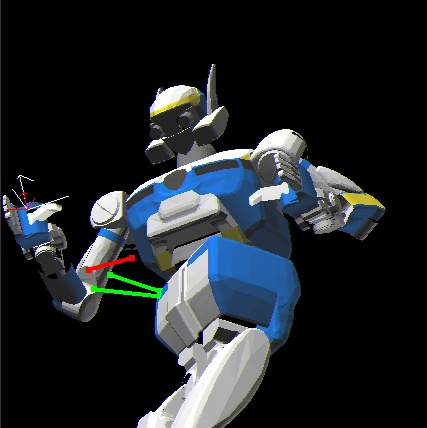
\includegraphics[width=0.50\columnwidth]{fig/collision-avoidance-example.jpg}
    \caption{Example of Collision Avoidance}
    \labfig{collision-avoidance-example}
  \end{center}
\end{figure}

%% PQP は SSV(Swept Sphere Volumes) を用い,三次元の物体同士の衝突判定,
%% 及び距離
%% 計算を高速に行う.ここで,SSV とは,点・線分・長方形の各形状プリミティ
%% ブを
%% 三次元的に膨張させて作成した BV(Bounding Volumes) セットであり,包含物
%% 体に
%% フィットした表現を可能とする特徴を持つ.
%% これら BV 要素同士の最短距離計算には,外部ボロノイ領域を考慮する,
%% Lin-Canny の
%% 最短距離計算アルゴリズム\cite{PQP:Lin91distance}を改良して用いる.
%% 二つの物体同士の距離計算は,各物体に対し,その物体の BV をノード
%% とするような探索木(BVH, Bounding Volume Hierarchies)を作成し,
%% 最短となる距離を再起的に計算していくことにより行う.
%% @INPROCEEDINGS{PQP:Lin91distance,
%%  author = {Ming C. Lin and John F. Canny},
%%  title = {A Fast Algorithm for Incremental Distance Calculation},
%%  booktitle = {In IEEE International Conference on Robotics and
%%    Automation},
%%  year = {1991},
%%  pages = {1008--1014}
%% }

%% 複数マニピュレータ・ヒューマノイドにおける安定な逆運動学求解に関して
\subsubsection{非ブロック対角ヤコビアンによる全身協調動作生成}
%%大きな対象物,重い対象物のマニピュレーションの際には,
%%単一マニピュレータだけではなく,複数のマニピュレータをもちい,
%%エンドエフェクタに限定しない接触点を設け動作を生成する必要がある.
%%本節では複数マニピュレータによる動作生成法を示す.
%%\subsection{重複リンクに応用可能な双腕協調逆運動学法}
%%\subsection{非ブロック対角ヤコビアンによる協調動作生成}
ヒューマノイドは枝分かれのある複雑な構造を持ち,
複数のマニピュレータで協調して動作を行う必要がある
(\reffig{duplicate-link}).

\begin{figure}[htb]
  \begin{center}
    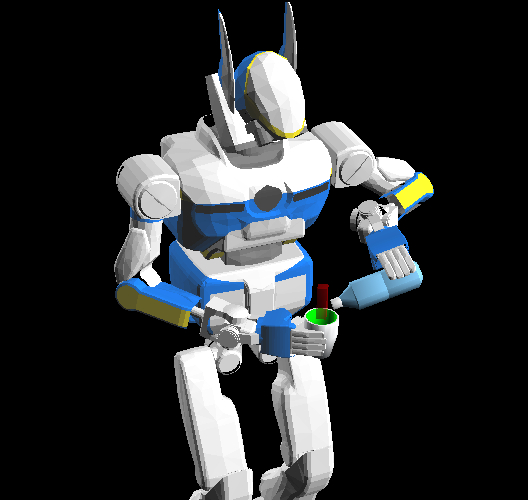
\includegraphics[width=0.49\columnwidth]{fig/normal.jpg}
    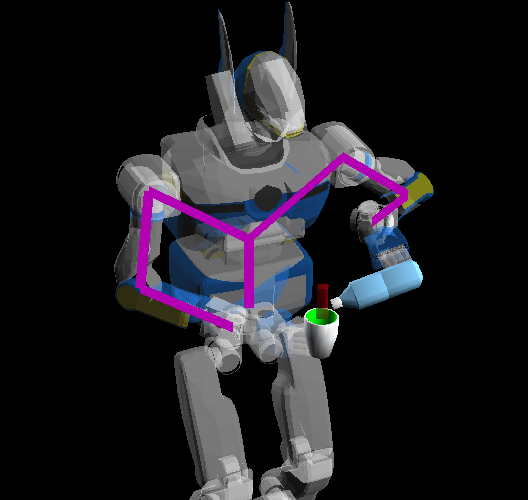
\includegraphics[width=0.49\columnwidth]{fig/linklist.jpg}
    \caption{Duplicate Link Sequence}
    \labfig{duplicate-link}
  \end{center}
\end{figure}

複数マニピュレータの動作例として,
\begin{itemize}
\item リンク間に重複がない場合\\
それぞれのマニピュレータについて
\refeq{inverse-kinematics}式を用いて関節角速度を求める.
もしくは,複数の式を連立した方程式(ヤコビアンはブロック対角行列となる)
を用いて関節角速度を求めても良い.
\item リンク間に重複がある場合\\
リンク間に重複がある場合は,
リンク間の重複を考慮したヤコビアンを考える必要がある.
例えば,双腕動作を行う場合,左腕のマニピュレータのリンク系列と
右腕のマニピュレータのリンク系列とで,体幹部リンク系列が重複し,
その部位は左右で協調して関節角速度を求める必要がある.
\end{itemize}
次節ではリンク間に重複がある場合の
非ブロック対角なヤコビアンの計算法
および
それを用いた関節角速度計算法を述べる
(前者の重複がない場合も以下の計算方法により後者の一部として計算可能で
ある).

\subsubsection{リンク間重複があるヤコビアン計算と関節角度計算}
%% マニピュレータをリンク系列で表した際に,
%% 複数のマニピュレータ系列に属するリンクがある場合
%% (すなわち重複するリンク,関節がある場合)での
%% ヤコビアンの関係式を導出し,それに基づく関節角速度計算を行う.
微分運動学方程式を求める際の条件を以下に示す.
\begin{itemize}
\item マニピュレータの本数 $L$本
\item 全関節数 $N$個
\item マニピュレータの先端速度・角速度ベクトル 
$[\bm{\xi}_0^T,...,\bm{\xi}_{L-1}^T]^T$
\item 各関節角速度ベクトル 
$[\bm{\dot{\theta}_0}^T,...,\bm{\dot{\theta}_{L-1}}^T]^T$
\item 関節の添字和集合 $S = \{0,\hdots,N-1\}$\\
ただし,マニピュレータ$i$の添字集合$S_i$を用いて$S$は
$S = S_0 \cup \hdots \cup S_{L-1}$と表せる.
\item $S$に基づく関節速度ベクトル $[\dot{\theta}_0, ..., \dot{\theta}_{N-1}]^T$
\end{itemize}
とする.

運動学関係式は\refeq{multi-manipulator-jacobi-eq}のようになる.

\begin{eqnarray}
\left[
\begin{array}{c}
\bm{\xi}_0 \\
\vdots\\
\bm{\xi}_{L-1}
\end{array}
\right]
=
\left[
\begin{array}{ccc}
\bm{J}_{0,0}   &        \hdots & \bm{J}_{0, N-1}\\
\vdots         &  \bm{J}_{i,j} & \vdots\\
\bm{J}_{L-1,0} &        \hdots & \bm{J}_{L-1, N-1}
\end{array}
\right]
\left[
\begin{array}{c}
\dot{\theta}_0\\
\vdots\\
\dot{\theta}_{N-1}
\end{array}
\right]
\labeq{multi-manipulator-jacobi-eq}
\end{eqnarray}

小行列$\bm{J}_{i,j}$は以下のように求まる.

\begin{numcases}
%%\label{basic-jacobian-column-of-virtual-joint}
{\bm{J}_{i,j}=} 
%% \left[
%% \begin{array}{ccc}
%% \bm{a}_j \times (\bm{p}_{end, i} - \bm{p}_j)\\
%% \bm{a}_j
%% \end{array}
%% \right]
\bm{J}_j
& if $j$-th joint $\in$ $i$-th link array\\
\bm{0} & otherwise
\end{numcases}
ここで,$\bm{J}_j$は\refeq{basic-jacobian-column-vector}のもの.

\refeq{multi-manipulator-jacobi-eq}を単一のマニピュレータの
逆運動学解法と同様にSR-Inverseを用いて関節角速度を
求めることができる.

ここでの非ブロック対角ヤコビアンの計算法は,
アーム・多指ハンドの動作生成
\footnote{
アーム・多指ハンド機構による把握と操り, 永井 清, 吉川 恒夫,
日本ロボット学会誌, vol. 13, no. 7, pp. 994-1005, 1995.
%ArmHand:Nagai:JRSJ95
}に
おいて登場する運動学関係式から求まるヤコビアンを
導出することが可能である.

%% 複数マニピュレータ・ヒューマノイドにおける安定な逆運動学求解に関して
\subsubsection{ベースリンク仮想ジョイントを用いた全身逆運動学法}
一般に関節数が$N$であるのロボットの運動を表現するためには
ベースリンクの位置姿勢と関節角自由度を合わせた$N+6$個の変数が必要であ
る.
ベースリンクとなる位置姿勢の変数を用いたロボットの運動の定式化は
宇宙ロボット\footnote{
%GeneralJacobian:Umetani:JRSJ89
一般化ヤコビ行列を用いた宇宙用ロボットマニピュレータの分解速度制御,
梅谷 陽二, 吉田 和哉,
日本ロボット学会誌, vol. 4, no. 7, pp. 63-73, 1989.
}だけでなく,
環境に固定されないヒューマノイドロボット
\footnote{
%FreeFloatingHumanoid:Luis:ICRA05
Control of Free-Floating Humanoid Robots Through Task Prioritization,
Luis Sentis and Oussama Khatib,
Proceedings of The 2005 IEEE International Conference on Robotics and Automation,
pp. 1718-1723, 2005
}の場合にも重要である.

ここでは
腕・脚といったマニピュレータに
ベースリンクに3自由度の直動関節と
3自由度の回転関節が仮想的に付随したマニピュレータ構成を考える
(\reffig{base-link-virtual-joint}).
上記の仮想的な6自由度関節を
本研究ではベースリンク仮想ジョイントと名づける.
ベースリンク仮想ジョイントを用いることにより
ヒューマノイドの腰が動き全身関節が駆動され,
運動学,ひいては動力学的な解空間が拡充されることが期待できる.
\begin{figure}[htb]
  \begin{center}
    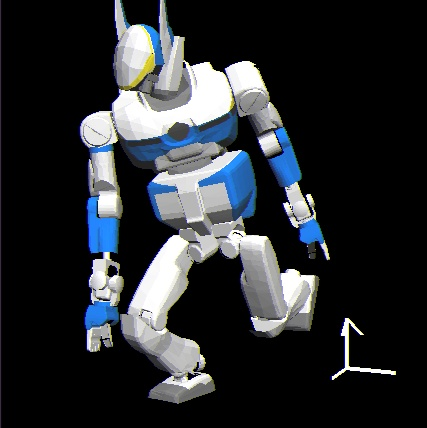
\includegraphics[width=0.49\columnwidth]{fig/6dof-manip-glview.jpg}
    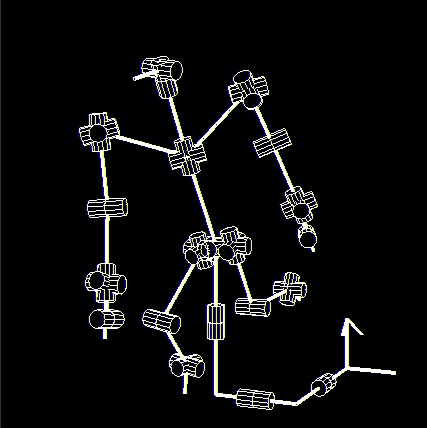
\includegraphics[width=0.49\columnwidth]{fig/6dof-manip-skelton.jpg}
    \caption{Concept of the Virtual Joint of the Base Link\newline
      (Left figure) Overview of the Robot Model\newline
      (Right figure) Skeleton Figure of Robot Model with the Virtual Joint
    }
    \labfig{base-link-virtual-joint}
  \end{center}
\end{figure}

%%\subsubsection{他の研究との比較}
%%運動学拘束に利用可能な変数としてのベースリンクの位置姿勢の利用を
%%\subsection{ベースリンク仮想ジョイントを用いた全身逆運動学法}
%%ベースリンク仮想ジョイントの位置姿勢の6自由度を求める計算をするための
%%ものである.
%%仮想ジョイント法の主たるコンセプトは,
%% ベースリンクの運動を規定する6自由度の速度・角速度情報$\bm{\xi_B}$を,
%% ベースリンクに3自由度の直動関節と
%% 3自由度の回転関節が付随したモデルで考える点である.

%%仮想ジョイント法は,速度情報と等価な式になる.l
%%違う点は,運動学解としてのルートリンク座標系決定を行う点.
%%ジョイントの定義=min maxがある.

%%\subsubsection{ベースリンク仮想ジョイントとassoc,parent-linkなどの関係について書く}

\subsubsection{ベースリンク仮想ジョイントヤコビアン}
ベースリンク仮想ジョイントのヤコビアンは
基礎ヤコビ行列の計算(\eqref{basic-jacobian-column-vector})
を利用し,
絶対座標系$x$,$y$,$z$軸の直動関節と
絶対座標系$x$,$y$,$z$軸回りの回転関節を
それぞれ連結した$6\times6$行列である.
%% \begin{numcases}
%% %%\label{basic-jacobian-column-of-virtual-joint}
%% {\bm{J}_j=}
%% \left[
%% \begin{array}{ccc}
%% \bm{e}_j\\
%% \bm{0}
%% \end{array}
%% \right]
%% & if linear joint, j = x, y, z \\
%% \left[
%% \begin{array}{ccc}
%% \bm{e}_j \times (\bm{p}_{end} - \bm{p}_B)\\
%% \bm{e}_j
%% \end{array}
%% \right]
%% & if rotational joint, j = x, y, z
%% \end{numcases}
%% ただし,
%% $\bm{e}_x=[1\ 0\ 0]^T$,
%% $\bm{e}_y=[0\ 1\ 0]^T$,
%% $\bm{e}_z=[0\ 0\ 1]^T$である.
ちなみに,並進・回転成分のルートリンク仮想ジョイントのヤコビアンは
以下のように書き下すこともできる.
\begin{eqnarray}
\labeq{virtual-joint-jacobian}
\bm{J}_{B,l} = 
\left[
\begin{array}{cc}
\bm{E}_3 &
-\hat{\bm{p}}_{B\to l}\\
\bm{0} & \bm{E}_3
\end{array}
\right]
\end{eqnarray}
%% \refeq{virtual-joint-jacobian}は
%% ルートリンクが動いた場合のエンドエフェクタに及ぼす
%% 速度・角速度ヤコビアン\cite{RMC:Kajita:JRSJ04}に他ならない.
%%\subsubsection{その他記号について}
$\bm{p}_{B\to l}$はベースリンク位置から添字$l$で表現する位置までの
差分ベクトルである.

% リンクのマスプロパティ追加法について述べる.

\subsubsection{マスプロパティ計算}
複数の質量・重心・慣性行列を統合し
単一の質量・重心・慣性行列の組
$[m_{new}, \bm{c}_{new}, \bm{I}_{new}]$
を計算する演算関数を次のように定義する.
\begin{equation}
[m_{new}, \bm{c}_{new}, \bm{I}_{new}]
= AddMassProperty(
[m_{1}, \bm{c}_{1}, \bm{I}_{1}]
,\hdots,
[m_{K}, \bm{c}_{K}, \bm{I}_{K}]
)
\end{equation}
これは次のような演算である.
\begin{equation}
m_{new} = \sum_{j=1}^{K}m_{j}
\end{equation}
\begin{equation}
\bm{c}_{new} = \frac{1}{m_{new}}\sum_{j=1}^{K} m_j \bm{c}_j
\end{equation}
\begin{equation}
\bm{I}_{new} = \sum_{j=1}^{K}
\left(
\bm{I}_j + m_j \bm{D}(\bm{c}_{j} - \bm{c}_{new})
\right)
\end{equation}
ここで,$\bm{D}(\bm{r})=\hat{\bm{r}}^T\hat{\bm{r}}$とする.
%%$\hat{\bm{r}}$は$\bm{r}$の外積と等価な歪対称行列である.

\subsubsection{運動量・角運動量ヤコビアン}
シリアルリンクマニピュレータを対象とし,
運動量・角運動量ヤコビアンを導出する.
運動量・原点まわりの角運動量を各関節変数で表現し,
その偏微分でヤコビアンの行を計算する.

第$j$関節の運動変数を$\theta_j$とする.
まず,回転・並進の1自由度関節を考える.
\begin{numcases}
{\bm{P}_j =}
\begin{array}{cl}
\bm{a}_j \dot{\theta}_j \times (\tilde{\bm{c}}_{j} - \bm{p}_j) \tilde{m}_j
& \text{if rotational joint}\\
\bm{a}_j \dot{\theta}_j \tilde{m}_j &
\text{if linear joint}
\end{array}
\end{numcases}
\begin{numcases}
{\bm{L}_j =}
\begin{array}{cl}
\tilde{\bm{c}}_{j} \bm{P}_j + \tilde{\bm{I}}_j \bm{a}_j \dot{\theta}_j
& \text{if rotational joint}\\
\bm{0} & \text{if linear joint}
\end{array}
\end{numcases}
ここで,
$[\tilde{m}_j, \tilde{\bm{c}}_j, \tilde{\bm{I}}_j]$は
AddMassProperty関数に第$j$関節の子リンクより
末端側のリンクのマスプロパティを与えたものであり,
実際には再帰計算により計算する\footnote{
%RMC:Kajita:IROS03
Resolved Momentum Control:Humanoid Motion Planning based on the Linear
and Angular Momentum,
S.Kajita, F.Kanehiro, K.Kaneko, K.Fujiwara, K.Harada, K.Yokoi,H.Hirukawa, 
In Proceedings of the 2003 IEEE/RSJ International Conference on Intelligent Robots and Systems (IROS'03),
pp. 1644-1650, 2003}.
これらを$\dot{\theta}_j$で割ることにより
ヤコビアンの各列ベクトルを得る.
\begin{numcases}
{\bm{m}_j =}
\begin{array}{cl}
\bm{a}_j \times (\tilde{\bm{c}}_{j} - \bm{p}_j) \tilde{m}_j
& \text{if rotational joint}\\
\bm{a}_j \tilde{m}_j & \text{if linear joint}
\end{array}
\end{numcases}
\begin{numcases}
{\bm{h}_j =}
\begin{array}{cl}
\tilde{\bm{c}}_{j} \times \bm{m}_j + \tilde{\bm{I}}_j \bm{a}_j
& \text{if rotational joint}\\
\bm{0} & \text{if linear joint}
\end{array}
\end{numcases}
これより慣性行列は次のように計算できる.
\begin{equation}
\bm{M}_{\dot{\bm{\theta}}}
=
[\bm{m}_1, \hdots, \bm{m}_{N}]
\end{equation}
\begin{equation}
\bm{H}_{\dot{\bm{\theta}}}
=
[\bm{h}_1, \hdots, \bm{h}_{N}]
-
\hat{\bm{p}}_{G} \bm{M}_{\dot{\bm{\theta}}}
\end{equation}
ここでは,全関節数を$N$とした.
また,ベースリンクは
直動関節$x$,$y$,$z$軸,
回転関節$x$,$y$,$z$軸を
もつと考え整理し,次のようになる.
\begin{eqnarray}
\left[
\begin{array}{c}
\bm{M}_{B}\\
\bm{H}_{B}
\end{array}
\right]
=
\left[
\begin{array}{cc}
M_{r} \bm{E}_3 & - M_{r} \hat{\bm{p}}_{B\to G}\\
\bm{0} & \tilde{\bm{I}}
\end{array}
\right]
\end{eqnarray}
これを用いて重心まわりの角運動量・運動量は次のようになる.
\begin{eqnarray}
%%\label{eq:org_rmc}
\left[
\begin{array}{c}
\bm{P}\\
\bm{L}
\end{array}
\right]
=
\left[
\begin{array}{cc}
\bm{M}_{B} & \bm{M}_{\dot{\bm{\theta}}}\\
\bm{H}_{B} & \bm{H}_{\dot{\bm{\theta}}}
\end{array}
\right]
\left[
\begin{array}{c}
\bm{\xi}_{B}\\
\dot{\bm{\theta}}
\end{array}
\right]
\end{eqnarray}
ここで
ヒューマノイドの全質量$M_{r}$,
重心位置$\bm{p}_{G}$,
慣性テンソル$\tilde{\bm{I}}$は次のように
全リンクのマスプロパティ演算より求める.
\begin{equation}
[M_{r}, \bm{p}_{G}, \tilde{\bm{I}}]
= AddMassProperty(
[m_{1}, \bm{c}_{1}, \bm{I}_{1}]
,\hdots,
[m_{N}, \bm{c}_{N}, \bm{I}_{N}]
)
\end{equation}

\subsubsection{重心ヤコビアン}
重心ヤコビアン%\{
%CogJacobian:Sugihara:IROS02
%}
は
重心速度と関節角速度の間のヤコビアンである.
本論文ではベースリンク仮想ジョイントを用いるため,
ベースリンクに6自由度関節がついたと考え
ベースリンク速度角速度・関節角速度の
重心速度に対するヤコビアンを重心ヤコビアンとして用いる.
具体的には,
ベースリンク成分$\bm{M}_{B}$と
使用関節について抜き出した成分$\bm{M}_{\dot{\bm{\theta}}}^{\prime}$
による運動量ヤコビアンを
全質量で割ることで重心ヤコビアンを計算する.
\begin{equation}
\bm{J}_{G} = 
\frac{1}{M_{r}}
\left[
\begin{array}{cc}
\bm{M}_{B} & \bm{M}_{\dot{\bm{\theta}}}^{\prime}
\end{array}
\right]
\end{equation}


\subsection{ロボットの動作生成プログラミング}
%% \subsubsection{逆運動学}

%% 与えられた目標リンク(例えば手先)の位置,姿勢からロボットの各関節角度を求
%% めることを逆運動学を解くという.その解き方には数値解法と解析解法がある
%% が,ここではより汎用的な数値解法のアルゴリズムを紹介する.

%% \begin{enumerate}
%% \item 目標リンクの位置姿勢($p^{ref},R^{ref}$)を設定する
%% \item 胴体から目標リンクまでの関節各度を並べたベクトルを$q$とする
%% \item 順運動学計算で注目するリンクの位置,姿勢($p,R$)を計算する
%% \item 位置・姿勢の誤差($\delta p,\delta R$) = ($p^{ref}-p, R^T
%%   R^{ref}$)を計算する
%% \item ($\delta p,\delta R$)が十分に小さければ終了
%% \item ($\delta p,\delta R$)が大きければ,これを小さくする関節角度修正
%%   量$\delta q$を計算する
%% \item $q = q + \delta q$として(3)に戻る.
%% \end{enumerate}

%% 位置姿勢の誤差($\delta p,\delta R$)が小さい,という条件は
%% 与えられた回転行列($R$)に対する角速度ベクトル($\omega$)を導入し
%% $err(\delta p,\delta R) =  ||\delta p||^2 + ||\delta \omega||^2$
%% がある閾値より小さい場合で判断できる.

%% \subsubsection{ヤコビアン}

%% 現在の状態から関節各度を微小単位$\delta q$動かした場合の位置姿勢の変化
%% 量との関係を
%% $
%%  \left[
%%  \begin{array}{c}
%%   \delta p \\
%%   \delta \omega
%%  \end{array}
%%  \right]
%%  = J \delta q
%% $
%% としたとき,Jをヤコビアンと呼ぶ.
%% Jの逆行列を使い
%% \[
%%  \delta q
%%  =
%%  J ^{-1}
%%  \left[
%%  \begin{array}{c}
%%   \delta p \\
%%   \delta \omega
%%  \end{array}
%%  \right]
%% \]
%% とすることで,手先の位置姿勢の誤差から,関節角度の修正量を計算する事が
%% 出来る.

\subsubsection{三軸関節ロボットを使ったヤコビアン,逆運動学の例}

%より複雑なロボットとして
3軸関節をもつロボットを定義し,
逆運動学やヤコビアンの計算例を紹介する.

ロボットの定義は以下の用になる.
{\baselineskip=10pt
\begin{verbatim}

(defclass 3dof-robot
  :super cascaded-link
  :slots (end-coords l1 l2 l3 l4 j1 j2 j3))
(defmethod 3dof-robot
  (:init ()
   (let (b)
     (send-super :init)

     (setq b (make-cube 10 10 20))
     (send b :locate #f(0 0 10))
     (send b :set-color :red)
     (setq l4 (instance bodyset-link :init (make-cascoords) :bodies (list b) :name 'l4))
     (setq end-coords (make-cascoords :pos #f(0 0 20)))
     (send l4 :assoc end-coords)
     (send l4 :locate #f(0 0 100))
     ;;
     (setq b (make-cube 10 10 100))
     (send b :locate #f(0 0 50))
     (send b :set-color :green)
     (setq l3 (instance bodyset-link :init (make-cascoords) :bodies (list b) :name 'l3))
     (send l3 :assoc l4)
     (send l3 :locate #f(0 0 100))
     ;;
     (setq b (make-cube 10 10 100))
     (send b :locate #f(0 0 50))
     (send b :set-color :blue)
     (setq l2 (instance bodyset-link :init (make-cascoords) :bodies (list b) :name 'l2))
     (send l2 :assoc l3)
     (send l2 :locate #f(0 0 20))
     ;;
     (setq b (body+ (make-cube 10 10 20 :pos #f(0 0 10)) (make-cube 300 300 2)))
     (send b :set-color :white)
     (setq l1 (instance bodyset-link :init (make-cascoords) :bodies (list b) :name 'l1))
     (send l1 :assoc l2)
     ;;
     (setq j1 (instance rotational-joint :init :name 'j1
                 :parent-link l1 :child-link l2 :axis :y :min -100 :max 100)
           j2 (instance rotational-joint :init  :name 'j2
                 :parent-link l2 :child-link l3 :axis :y :min -100 :max 100)
           j3 (instance rotational-joint :init  :name 'j3
                 :parent-link l3 :child-link l4 :axis :y :min -100 :max 100))
     ;;
     (setq links (list l1 l2 l3 l4))
     (setq joint-list (list j1 j2 j3))
     ;;
     (send self :init-ending)
     self))
  (:end-coords (&rest args) (forward-message-to end-coords args))
  )
\end{verbatim}
}

ここではロボットの手先の座標を\verb|end-coords|というスロット変数に格
納し,さらにこれにアクセスするためのメソッドを用意してある.

これまでと同様,
{\baselineskip=10pt
\begin{verbatim}
(setq r (instance 3dof-robot :init))
(objects (list r))
(send r :angle-vector #f(30 30 30))
\end{verbatim}
}
としてロボットモデルの生成,表示,関節角度の指定が可能である.
さらに,

{\baselineskip=10pt
\begin{verbatim}
(send (send r :end-coords) :draw-on :flush t)
\end{verbatim}
}

とすると,ロボットの\verb|end-coords|(端点座標系)の表示が可能であるが,
マウスイベントが発生すると消えてしまう.恒久的に表示するためには

{\baselineskip=10pt
\begin{verbatim}
(objects (list r (send r :end-coords)))
\end{verbatim}
}

とするとよい.

次に,ヤコビアン,逆運動学の例を示す.まず基本になるのが,
{\baselineskip=10pt
\begin{verbatim}
(send r :link-list (send r :end-coords :parent))
\end{verbatim}
}
として得られるリンクのリストである.これはロボットのルート(胴体)から
引数となるリンクまでのたどれるリンクを返す.

\verb|:calc-jacobian-from-link-list|メソッドはリンクのリストを引数にと
り,この各リンクに存在するジョイント(関節)に
対応するヤコビアンを計算することができる.
また,\verb|:move-target|キーワード引数でエンドエフェクタの座標系を
指定してる.その他のキーワード引数については後述する.

{\baselineskip=10pt
\begin{verbatim}
(dotimes (i 100)
  (setq j (send r :calc-jacobian-from-link-list
                (send r :link-list (send r :end-coords :parent))
                :move-target (send r :end-coords)
                :rotation-axis t
                :translation-axis t))
  (setq j# (sr-inverse j))
  (setq da (transform j# #f(1 0 0 0 0 0)))
  ;;(setq da (transform j# #f(0 0 0 0 -1 0)))
  (send r :angle-vector (v+ (send r :angle-vector) da))
  (send *irtviewer* :draw-objects)
  )
\end{verbatim}
}

ここではリンクの長さ(ジョイントの数)は3個なので6行3列のヤコビアン(\verb|j|)が
計算される.これの逆行列(\verb|j#|)を作り,位置姿勢の6自由度の目標速度・角速度
(\verb|#f(1 0 0 0 0 0)|)を与えると,それに対応する関節速度(\verb|da|)
が計算でき,これを現在の関節角度に足している
(\verb|(v+ (send r :angle-vector) da)|).


次に,ロボットの端点作業の位置は合わせるが姿勢は拘束せず任意のままでよい,とい
う場合の例を示す.ここでは,\verb|:calc-jacobian-from-link-list|のオプ
ショナル引数として\verb|:rotation-axis|, \verb|:translation-axis|
があり,それぞれ位置,姿勢での拘束条件を示す.
\verb|t|は三軸拘束,\verb|nil|は拘束なし,その他に\verb|:x|,
\verb|:y|, \verb|:z|を指定することができる.

{\baselineskip=10pt
\begin{verbatim}
(setq translation-axis t)
(setq rotation-axis nil)
(dotimes (i 2000)
  (setq j (send r :calc-jacobian-from-link-list
                (send r :link-list (send r :end-coords :parent))
                :move-target (send r :end-coords)
                :rotation-axis rotation-axis
                :translation-axis translation-axis))
  (setq j# (sr-inverse j))
  (setq c (make-cascoords :pos (float-vector (* 100 (sin (/ i 500.0))) 0 200)))
  (setq dif-pos (send (send r :end-coords) :difference-position c))
  (setq da (transform j# dif-pos))
  (send r :angle-vector (v+ (send r :angle-vector) da))
  (send *irtviewer* :draw-objects :flush nil)
  (send c :draw-on :flush t)
  )
\end{verbatim}
}

ここでは位置の三軸のみを拘束した3行3列のヤコビアンを計算し,これの
逆行列からロボットの関節に速度を与えている.さらに,ここでは
{\baselineskip=10pt
\begin{verbatim}
  (send *irtviewer* :draw-objects :flush nil)
\end{verbatim}
}
として\verb|*irtviewer*|に画面を描画しているが,実際に
ディスプレイに表示するフラッシュ処理は行わず,その次の行の
{\baselineskip=10pt
\begin{verbatim}
  (send c :draw-on :flush t)
\end{verbatim}
}
で目標座標は表示し,かつフラッシュ処理を行っている.

上記の計算をまとめた逆運動学メソッドが\verb|:inverse-kinematics|である.
第一引数に目標座標系を指定し,ヤコビアン計算のときと同様にキーワード
引数で
\verb|:move-target|, \verb|:translation-axis|, \verb|:rotation-axis|
を指定する.
また,\verb|:debug-view|キーワード引数に\verb|t|を与えると計算中の様
子をテキスト並びに視覚的に提示してくれる.
{\baselineskip=10pt
\begin{verbatim}
(setq c (make-cascoords :pos #f(100 0 0) :rpy (float-vector 0 pi 0)))
(send r :inverse-kinematics  c
      :link-list (send r :link-list (send r :end-coords :parent))
      :move-target (send r :end-coords)
      :translation-axis t
      :rotation-axis t
      :debug-view t)
\end{verbatim}
}

逆運運動学が失敗する場合のサンプルとして以下のプログラムを見てみよう.
{\baselineskip=10pt
\begin{verbatim}
(dotimes (i 400)
  (setq c (make-cascoords
             :pos (float-vector (+ 100 (* 80 (sin (/ i 100.0)))) 0 0)
             :rpy (float-vector 0 pi 0)))
  (send r :inverse-kinematics  c
        :link-list (send r :link-list (send r :end-coords :parent))
        :move-target (send r :end-coords) :translation-axis t  :rotation-axis t)
  (x::window-main-one)
  (send *irtviewer* :draw-objects :flush nil)
  (send c :draw-on :flush t)
  )
\end{verbatim}
}

このプログラムを実行すると以下のようなエラーが出てくる.
{\baselineskip=10pt
\begin{verbatim}
;; inverse-kinematics failed.
;; dif-pos : #f(11.7826 0.0 0.008449)/(11.7826/1)
;; dif-rot : #f(0.0 2.686130e-05 0.0)/(2.686130e-05/0.017453)
;;  coords : #<coordinates #X4bcccb0  0.0 0.0 0.0 / 0.0 0.0 0.0>
;;  angles : (14.9993 150 15.0006)
;;    args : ((#<cascaded-coords #X4b668a0  39.982 0.0 0.0 / 3.142 1.225e-16 3.14
2>) :link-list (#<bodyset-link #X4cf8e60 l2  0.0 0.0 20.0 / 0.0 0.262 0.0> #<body
set-link #X4cc8008 l3  25.866 0.0 116.597 / 3.142 0.262 3.142> #<bodyset-link #X4
c7a0d0 l4  51.764 0.0 20.009 / 3.142 2.686e-05 3.142>) :move-target;; #<cascaded-
coords #X4c93640  51.764 0.0 0.009 / 3.142 2.686e-05 3.142> :translation-axis t :
rotation-axis t)
\end{verbatim}
}

これは,関節の駆動範囲の制限から目標位置に手先が届かない状況である.
このような場面では,例えば,手先の位置さえ目標位置に届けばよく姿勢を
無視してよい場合\verb|:rotation-axis nil|と指定することができる.

また,\verb|:thre|や\verb|:rthre|を使うことで逆運動学計算の終了条件で
ある位置姿勢の誤差を指定することができる.正確な計算が求められていない
状況ではこの値をデフォルトの\verb|1|, \verb|(deg2rad 1)|より大きい値を
利用するのもよい.

また,逆運動学の計算に失敗した場合,デフォルトでは逆運動学計算を始める
前の姿勢まで戻るが,\verb|:revert-if-fail|というキーワード引数をnilと指定
すると,指定されたの回数の計算を繰り替えしたあと,その姿勢のまま関数か
ら抜けてくる.指定の回数もまた,\verb|:stop|というキーワード引数で指
定することができる.

{\baselineskip=10pt
\begin{verbatim}
(setq c (make-cascoords :pos #f(300 0 0) :rpy (float-vector 0 pi 0)))
(send r :inverse-kinematics  c
      :link-list (send r :link-list (send r :end-coords :parent))
      :move-target (send r :end-coords)
      :translation-axis t
      :rotation-axis nil
      :revert-if-fail nil)
\end{verbatim}
}

\subsubsection{irteusのサンプルプログラムにおける例}

cascaded-coordsクラスでは
\begin{itemize}
\item (:link-list (to \&optional form))
\item (:calc-jacobian-from-link-list (link-list \&key move-target
  (rotation-axis nil)))
\end{itemize}
というメソッドが用意されている.

前者はリンクを引数として,ルートリンクからこのリンクまでの経路を計算し,
リンクのリストとして返す.後者はこのリンクのリストを引数とし,
move-target座標系をに対するヤコビアンを計算する.

concatenate result-type a bは a bを
連結しresult-type型に変換し返し,scale a b はベクトルbの全ての要素をス
カラーa倍し,matrix-logは行列対数関数を計算する.

{\baselineskip=10pt
\begin{verbatim}
(if (not (boundp '*irtviewer*)) (make-irtviewer))

(load "irteus/demo/sample-arm-model.l")
(setq *sarm* (instance sarmclass :init))
(send *sarm* :reset-pose)
(setq *target* (make-coords :pos #f(350 200 400)))
(objects (list *sarm* *target*))

(do-until-key
  ;; step 3
  (setq c (send *sarm* :end-coords))
  (send c :draw-on :flush t)
  ;; step 4
  ;; step 4
  (setq dp (scale 0.001 (v- (send *target* :worldpos) (send c :worldpos))) ;; mm->m
        dw (matrix-log (m* (transpose (send c :worldrot)) (send *target* :worldrot))))
  (format t "dp = ~7,3f ~7,3f ~7,3f, dw = ~7,3f ~7,3f ~7,3f~%"
          (elt dp 0) (elt dp 1) (elt dp 2)
          (elt dw 0) (elt dw 1) (elt dw 2))
  ;; step 5
  (when (< (+ (norm dp) (norm dw)) 0.01) (return))
  ;; step 6
  (setq ll (send *sarm* :link-list (send *sarm* :end-coords :parent)))
  (setq j (send *sarm* :calc-jacobian-from-link-list
                ll :move-target (send *sarm* :end-coords)
                :trnaslation-axis t :rotation-axis t))
  (setq q (scale 1.0 (transform (pseudo-inverse j) (concatenate float-vector dp dw))))
  ;; step 7
  (dotimes (i (length ll))
    (send (send (elt ll i) :joint) :joint-angle (elt q i) :relative t))
  ;; draw
  (send *irtviewer* :draw-objects)
  (x::window-main-one))
\end{verbatim}
}

実際のプログラミングでは:inverse-kinematicsというメソッドが用意されて
おり,ここでは特異点や関節リミットの回避,あるいは自己衝突回避等の機能
が追加されている.

\subsubsection{実際のロボットモデル}

実際のロボットや環境を利用した実践的なサンプルプログラムを見てみよう.

まず,最初はロボットや環境のモデルファイルを読み込む.これらのファイル
は\${EUSDIR}/modelsに,これらのファイルをロードしインスタンスを生成す
るプログラムは以下のように書くことができる.\verb|(room73b2)|や
\verb|(h7)|はこれらのファイル内で定義されている関数である.
ロボットのモデル(\verb|robot-model|)は\verb|irtrobot.l|ファイルで定義
されており,\verb|cascaded-link|クラスの子クラスになっている.
ロボットとは\verb|larm,rarm,lleg,rleg,head|のリンクのツリーからなる
ものとして定義されており,
\verb|(send *robot* :larm)|や\verb|(send *robot* :head)|として
ロボットのリム(limb)にアクセスでき,右手の逆運動学,左手の逆運動学等と
いう利用方法が可能になっている.

{\baselineskip=10pt
\begin{verbatim}
(load "models/room73b2-scene.l")
(load "models/h7-robot.l")
(setq *room* (room73b2))
(setq *robot* (h7))
(objects (list *robot* *room*))
\end{verbatim}
}

ロボットには\verb|:reset-pose|というメソッドがありこれで初期姿勢をとる
ことができる.
{\baselineskip=10pt
\begin{verbatim}
(send *robot* :reset-pose)
\end{verbatim}
}

次に,ロボットを部屋の中で移動させたい.部屋内の代表的な座標は
\verb|(send *room* :spots)|で取得できる.この中から目的の座標を得る
場合はその座標の名前を引数として\verb|:spot|メソッドを呼び出す.
ちなみに,このメソッドの定義は\verb|prog/jskeus/irteus/irtscene.l|
にあり
{\baselineskip=10pt
\begin{verbatim}
(defmethod scene-model
  (:spots
   (&optional name)
   (append
    (mapcan
     #'(lambda(x)(if (derivedp x scene-model) (send x :spots name) nil))
     objs)
    (mapcan #'(lambda (o)
		(if (and (eq (class o) cascaded-coords)
			 (or (null name) (string= name (send o :name))))
		    (list o)))
	    objs)))
  (:spot
   (name)
   (let ((r (send self :spots name)))
     (case (length r)
       (0 (warning-message 1 "could not found spot(~A)" name) nil)
       (1 (car r))
       (t (warning-message 1 "found multiple spot ~A for given name(~A)" r name) (car r)))))
  )
\end{verbatim}
}
となっている.

ロボットもまた\verb|coordinates|クラスの子クラスなので\verb|:move-to|
メソッドを利用できる.また,このロボットの原点は腰にあるので足が地面に
つくように\verb|:locate|メソッドを使って移動する.
{\baselineskip=10pt
\begin{verbatim}
(send *robot* :move-to (send *room* :spot "cook-spot") :world)
(send *robot* :locate #f(0 0 550))
\end{verbatim}
}

現状では\verb|*irtviewer*|の画面上でロボットが小さくなっているので,
以下のメソッド利用し,ロボットが画面いっぱいになるように調整する.
{\baselineskip=10pt
\begin{verbatim}
(send *irtviewer* :look-all
      (geo::make-bounding-box
       (flatten (send-all (send *robot* :bodies) :vertices))))
\end{verbatim}
}

次に環境中の物体を選択する.ここでは\verb|:object|メソッドを利用する.
これは,\verb|:spots, :spot|と同様の振る舞いをするため,
どのような物体があるかは,\verb|(send-all (send *room* :objects) :name)|
として知ることができる.
\verb|room73b2-kettle|の他に
\verb|room73b2-mug-cup|や\verb|room73b2-knife|等を利用するとよい.

{\baselineskip=10pt
\begin{verbatim}
(setq *kettle* (send *room* :object "room73b2-kettle"))
\end{verbatim}
}

環境モデルの初期化直後は物体は部屋にassocされているため,以下の用に
親子関係を解消しておく.こうしないと物体を把持するなどの場合に問題が生
じる.
{\baselineskip=10pt
\begin{verbatim}
(if (send *kettle* :parent) (send (send *kettle* :parent) :dissoc *kettle*))
\end{verbatim}
}

ロボットの視線を対象物に向けるためのメソッドとして以下のようなものがあ
る.
{\baselineskip=10pt
\begin{verbatim}
(send *robot* :head :look-at (send *kettle* :worldpos))
\end{verbatim}
}

対象物体には,その物体を把持するための利用したらよい座標系が
\verb|:handle|メソッドとして記述されている場合がある.このメソッドは
リストを返すため以下の様に\verb|(car (send *kettle* :handle))|として
その座標系を知ることができる.この座標がどこにあるか確認するためには
\verb|(send (car (send *kettle* :handle)) :draw-on :flush t)|とすると
よい.

したがってこの物体手を伸ばすためには
{\baselineskip=10pt
\begin{verbatim}
(send *robot* :larm :inverse-kinematics
      (car (send *kettle* :handle))
      :link-list (send *robot* :link-list (send *robot* :larm :end-coords :parent))
      :move-target (send *robot* :larm :end-coords)
      :rotation-axis :z
      :debug-view t)
\end{verbatim}
}
となる.

ここで,ロボットの手先と対象物体の座標系を連結し,
{\baselineskip=10pt
\begin{verbatim}
(send *robot* :larm :end-coords :assoc *kettle*)
\end{verbatim}
}

以下の様にして世界座標系で100[mm]持ち上げることができる.
{\baselineskip=10pt
\begin{verbatim}
(send *robot* :larm :move-end-pos #f(0 0 100) :world
        :debug-view t :look-at-target t)
\end{verbatim}
}
\verb|:look-at-target|は移動中に首の向きを常に対象を見つづけるようにす
るという指令である.

\subsubsection{inverse-kinematicsのtarget-coordsに関数を指定する例}

\begin{figure}[htb]
  \begin{center}
    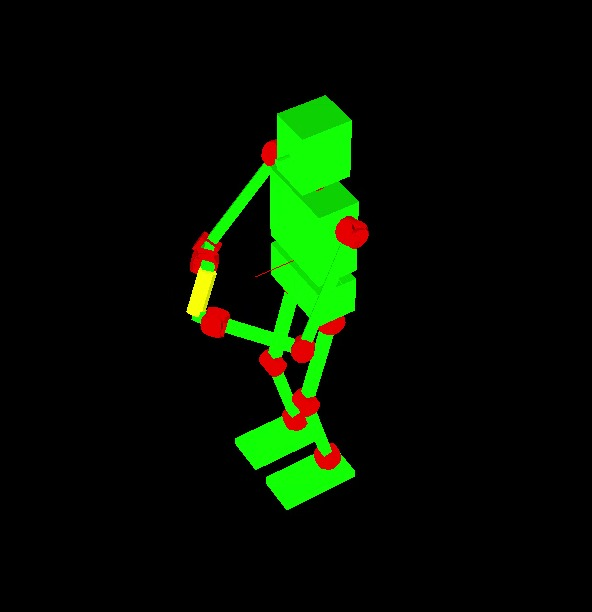
\includegraphics[width=0.49\columnwidth]{fig/dual-arm-ik.jpg}
    \caption{Example of Dual Arm InverseKinematics}
    \labfig{dual-arm-ik}
  \end{center}
\end{figure}

:inverse-kinematicsの引数target-coordsは\verb|coordinates|クラス以外に
\verb|coordinates|クラスを返す関数を指定することができる。
以下に示すプログラムは2つの腕を利用してカクテルをふる動作を行うものである(\reffig{dual-arm-ik})。

{\baselineskip=10pt
\begin{verbatim}
(load "irteus/demo/sample-robot-model.l")
(setq *robot* (instance sample-robot :init))
(setq *obj* (make-cylinder 20 100))
(send *obj* :set-color #f(1 1 0))
(send *robot* :reset-pose)
(objects (list *robot* *obj*))

(send *robot* :inverse-kinematics
      (list (make-coords :pos #f(400 0 0)))
      :move-target
      (list (send *robot* :larm :end-coords))
      :link-list
      (list (send *robot* :link-list
                  (send (send *robot* :larm :end-coords) :parent)
                  (car (send *robot* :larm :links))))
      :translation-axis (list t)
      :rotation-axis (list nil))

(let* ((cnt 0.0))
  (do-until-key
   (incf cnt 0.1)
   (send *robot* :inverse-kinematics
         (list (make-coords :pos (float-vector (+ 400 (* 100 (sin cnt))) (* 50 (cos cnt)) 0))
               #'(lambda ()
                   (send (send (send *robot* :larm :end-coords) :copy-worldcoords)
                         :translate #f(0 0 100) :local)))
         :move-target
         (list (send *robot* :larm :end-coords)
               (send *robot* :rarm :end-coords))
         :link-list
         (list (send *robot* :link-list
                     (send (send *robot* :larm :end-coords) :parent)
                     (car (send *robot* :larm :links)))
               (send *robot* :link-list
                     (send (send *robot* :rarm :end-coords) :parent)
                     (car (send *robot* :rarm :links))))
         :translation-axis (list :z t)
         :rotation-axis (list nil :z))
   (send *obj* :newcoords (send (send *robot* :larm :end-coords) :copy-worldcoords))
   (send *irtviewer* :draw-objects)))
\end{verbatim}
}

{\baselineskip=10pt
\begin{verbatim}
         (list (make-coords :pos (float-vector (+ 400 (* 100 (sin cnt))) (* 50 (cos cnt)) 0))
               #'(lambda ()
                   (send (send (send *robot* :larm :end-coords) :copy-worldcoords)
                         :translate #f(0 0 100) :local)))
\end{verbatim}
}

の行で実際にtarget-coordsに関数を指定している。
この例では、まずカクテルを持つ左手の位置を最初に決める。この時に
\verb|:translation-axis :z|, \verb|:rotation-axis nil|となっているため、
z方向の移動量と回転方向は左手の逆運動学の計算に考慮されない。
そして、決まった左手の位置に対して関数が評価されることで
手先のlocal座標から見てz方向に100の位置に対して右手の位置が決まる。
この時、右手の拘束条件は\verb|:translation-axis t|, \verb|:rotation-axis :z|となっ
ているためz方向、つまりカクテルの長さ方向を軸としてその軸に対する回転は許した条
件で逆運動学を解くことになる。
このように、拘束条件を踏まえて逆運動学を解きたい場合にはtarget-coordsを関数とし
て扱うことが必要になる。

\subsubsection{重心位置を考慮したfullbody-inverse-kinematicsの例}
\begin{figure}[htb]
  \begin{center}
    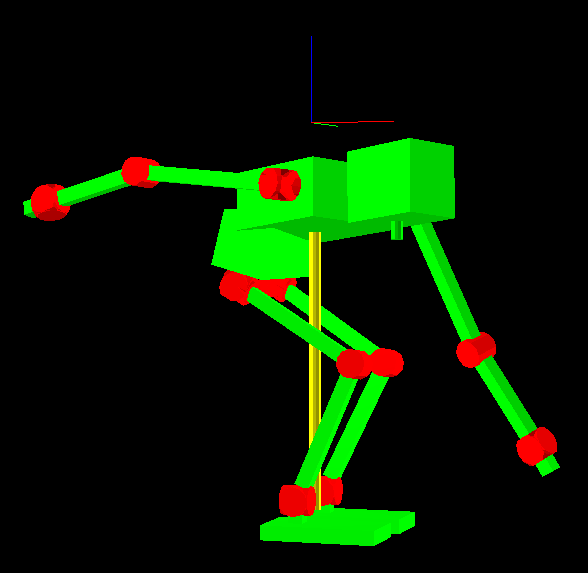
\includegraphics[width=0.49\columnwidth]{fig/full-body-ik.png}
    \caption{Example of InverseKinematics with root link virtual joint}
    \labfig{full-body-ik}
  \end{center}
\end{figure}
:fullbody-inverse-kinematicsはロボットの関節に加えてベースリンク仮想ジョイントを駆動した
逆運動学を解く関数である。以下に示すプログラムは、両足を地面に固定し、重心を両足の上に
位置させた状態で、左手を目標に到達させる動作を行うものである。
{\baselineskip=10pt
\begin{verbatim}
(load "irteus/demo/sample-robot-model.l")
(setq *robot* (instance sample-robot :init))
(send *robot* :reset-pose)
(setq *obj* (make-cylinder 10 600))
(send *obj* :rotate pi :x)
(send *obj* :set-color #f(1 1 0))
(objects (list *robot* *obj*))

(let* ((rleg-coords (send *robot* :rleg :end-coords :copy-worldcoords))
       (lleg-coords (send *robot* :lleg :end-coords :copy-worldcoords)))
   (send *robot* :fullbody-inverse-kinematics
         (list rleg-coords
               lleg-coords
               (make-coords :pos (float-vector 400 100 -600)))
         :move-target
         (list (send *robot* :rleg :end-coords)
               (send *robot* :lleg :end-coords)
               (send *robot* :larm :end-coords))
         :link-list
         (list (send *robot* :link-list (send *robot* :rleg :end-coords :parent))
               (send *robot* :link-list (send *robot* :lleg :end-coords :parent))
               (send *robot* :link-list (send *robot* :larm :end-coords :parent)))
         :translation-axis (list t t t)
         :rotation-axis (list t t nil)
         :target-centroid-pos (midpoint 0.5 (send *robot* :rleg :end-coords :worldpos)
                                            (send *robot* :lleg :end-coords :worldpos))
         :cog-translation-axis :z)
      (send *obj* :locate (send *robot* :centroid) :world)
      (send *irtviewer* :draw-objects))
\end{verbatim}
}

{\baselineskip=10pt
\begin{verbatim}
(list rleg-coords
      lleg-coords
      (make-coords :pos (float-vector 400 100 -600)))
\end{verbatim}
}
の行でtarget-coordsに右足、左足、左手の目標位置姿勢を指定している。
右足、左足は動かさないため、現在の座標をコピーしたものを与えている。
このときに、\verb|:translation-axis (list t t t)|, \verb|:rotation-axis (list t t nil)|
となっているため、右足、左足は位置姿勢を完全に拘束し、左手は姿勢の
回転は許した条件で逆運動学を解くことになる。

{\baselineskip=10pt
\begin{verbatim}
:target-centroid-pos (midpoint 0.5 (send *robot* :rleg :end-coords :worldpos)
                                   (send *robot* :lleg :end-coords :worldpos))
:cog-translation-axis :z)
\end{verbatim}
}
の行では重心の逆運動学を指定しており、\verb|:cog-translation-axis :z|で
z方向の重心の移動は許した状態で\verb|:target-centroid-pos|で目標位置として
両足の中間の座標を与えることによって、重心のxy座標を両足の中間に一致させる
条件のもとで逆運動学を解くことになる。

\subsubsection{外力を考慮したfullbody-inverse-kinematicsを解く例}
\begin{figure}[htb]
  \begin{center}
    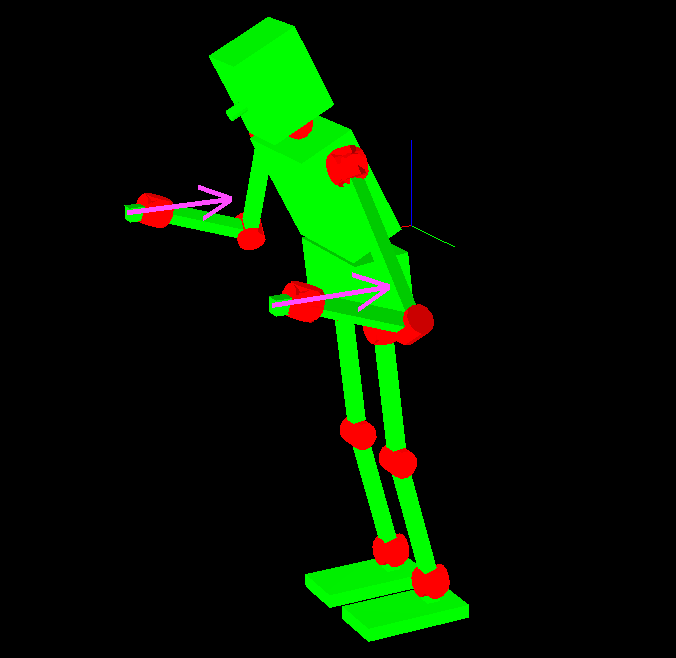
\includegraphics[width=0.49\columnwidth]{fig/static-balance-ik.png}
    \caption{Example of InverseKinematics with external force}
    \labfig{static-balance-ik}
  \end{center}
\end{figure}
ロボットが外力、外モーメントを受ける場合、外力による足裏まわりのモーメントと
釣り合うようにロボットの重心をオフセットすることによって、バランスをとることができる。
以下に示すプログラムは両手に外力、外モーメントが加わる場合に、両手両足を目標の位置に
到達させかつバランスが取れる姿勢を逆運動学によって求めるものである。

{\baselineskip=10pt
\begin{verbatim}
(load "irteus/demo/sample-robot-model.l")
(setq *robot* (instance sample-robot :init))
(send *robot* :reset-pose)
(setq *obj* (make-cylinder 10 600))
(objects (list *robot*))

(let* ((force-list '(#f(-20 0 0) #f(-20 0 0)))
       (moment-list '(#f(10 0 0) #f(10 0 0))))

  (send *robot* :fullbody-inverse-kinematics
        (list (send *robot* :rleg :end-coords :copy-worldcoords)
              (send *robot* :lleg :end-coords :copy-worldcoords)
              (make-coords :pos #f(400 -300 0))
              (make-coords :pos #f(400 300 0)))
        :move-target (mapcar #'(lambda (x)
                                 (send *robot* x :end-coords))
                             (list :rleg :lleg :rarm :larm))
        :link-list (mapcar #'(lambda (x)
                               (send *robot* :link-list (send *robot* x :end-coords :parent)))
                           (list :rleg :lleg :rarm :larm))
        :centroid-offset-func #'(lambda () (send *robot* :calc-static-balance-point
                                             :force-list force-list
                                             :moment-list moment-list))
        :target-centroid-pos (midpoint 0.5 (send *robot* :rleg :end-coords :worldpos)
                                            (send *robot* :lleg :end-coords :worldpos))
        :cog-translation-axis :z)
  (send *irtviewer* :draw-objects)

  ;; draw force
  (mapcar
   #'(lambda (f cc)
       (let* ((prev-color (send *viewer* :viewsurface :color))
              (prev-width (send *viewer* :viewsurface :line-width)))
         (send *viewer* :viewsurface :color #F(1 0.3 1))
         (send *viewer* :viewsurface :line-width 5)
         (send *irtviewer* :viewer :draw-arrow
               (send cc :worldpos)
               (v+ (send cc :worldpos) (scale 10 f)))
         (send *viewer* :viewsurface :color prev-color)
         (send *viewer* :viewsurface :line-width prev-width)))
   force-list
   (list (send *robot* :rarm :end-coords)
         (send *robot* :larm :end-coords)))
  (send *irtviewer* :viewer :viewsurface :flush)
  )
\end{verbatim}
}

この例では、
{\baselineskip=10pt
\begin{verbatim}
:centroid-offset-func #'(lambda () (send *robot* :calc-static-balance-point
                                     :force-list force-list
                                     :moment-list moment-list))
\end{verbatim}
}
の行で外力、外モーメントを考慮している。force-listは右手に作用する外力と左手に作用する外力のリスト、force-listは右手に作用する外モーメントと左手に作用する外モーメントのリストであり、単位はそれぞれ[N]、[Nm]である。:calc-static-balance-pointは、現在の両手の位置に作用する外力外モーメントと現在の重心の位置に作用する重力に対してバランスが取れる足裏圧力中心の位置を返す関数である。:centroid-offset-funcは\verb|float-vector|クラスを返す関数を指定することができ、現在の重心位置の代わりにこの関数の返り値を用いて目標重心位置との距離に応じた逆運動学を解く。\verb|:cog-translation-axis :z|でz方向の重心の移動は許した状態で\verb|:target-centroid-pos|で目標重心位置として両足の中間の座標を与えることによって、:centroid-offset-funcの返り値、即ちバランスが取れる足裏圧力中心のxy座標を両足の中間に一致させる逆運動学を解くことになる。

 \subsection{ロボットモデル}

ロボットの身体はリンクとジョイントから構成されるが、それぞれ
\verb|bodyset-link|と\verb|joint|クラスを利用しモデル絵を作成する。ロ
ボットの身体はこれらの要素を含んだ\verb|cascaded-link|という,連結リン
クとしてモデルを生成する.

実際には\verb|joint|は抽象クラスであり
\verb|rotational-joint|,\verb|linear-joint|,
\verb|wheel-joint|,\verb|omniwheel-joint|,
\verb|sphere-joint|を選択肢、また四肢を持つロボットの場合は
\verb|cascaded-link|
ではなく\verb|robot-model|クラスを利用する。

  \input{irtmodel-func}
  \input{irtgeo-func}
  \input{irtrobot-func}
 \subsection{センサモデル}
  \input{irtsensor-func}
 \subsection{環境モデル}
  \input{irtscene-func}
 \subsection{動力学計算・歩行動作生成}
  \input{irtdyna-func}

%% irtrobot.l
%% irtmodel.l
%% irtsensor.l
%% irtscene.l
%% irtdyna.l

\section{ロボットビューワ}
 \input{irtviewer-func}

\section{干渉計算}

干渉計算には2組の幾何モデルが交差するかを判定する物である.
irteusではノースカロライナ大学のLin氏らのグループにより開発されたPQPを
他言語インターフェースを介して利用できるようにしてある.
(他の干渉計算ソフトウェアパッケージについてはhttp://gamma.cs.unc.edu/research/collision/に詳しい.)
PQPは
(1)2つのモデルが交差するかを判定する衝突検出,
(2)2つのモデル間の最初距離を算出する距離計算,
(3)2つのモデルがある距離以下であるかを判定する近接検証,
等の3つ機能を提供する.

PQPソフトウェアパッケージの使い方はirteus/PQP/README.txtに
書いてあり,irteus/PQP/src/PQP.hを読むことで理解できるようになって
いる.

\subsection{irteusからPQPの呼び出し}

irteusでPQPを使うためのファイルは
CPQP.C, euspqp.c, pqp.l
からなる.
2つの幾何モデルが衝突してしるか否かを判定するためには,

{\baselineskip=10pt
\begin{verbatim}
(defun pqp-collision-check (model1 model2
				       &optional (flag PQP_FIRST_CONTACT) &key (fat 0) (fat2 nil))
  (let ((m1 (get model1 :pqpmodel))  (m2 (get model2 :pqpmodel))
        (r1 (send model1 :worldrot)) (t1 (send model1 :worldpos))
        (r2 (send model2 :worldrot)) (t2 (send model2 :worldpos)))
    (if (null fat2) (setq fat2 fat))
    (if (null m1) (setq m1 (send model1 :make-pqpmodel :fat fat)))
    (if (null m2) (setq m2 (send model2 :make-pqpmodel :fat fat2)))
    (pqpcollide r1 t1 m1 r2 t2 m2 flag)))
\end{verbatim}
}
を呼び出せば良い.
r1,r1,r2,t1はそれぞれの物体の並進ベクトル,回転行列となり,
(get model1 :pqpmodel)でPQPの幾何モデルへのポインタを参照する.
このポインタは:make-pqpmodelメソッドの中で以下のよう計算される.
{\baselineskip=10pt
\begin{verbatim}
(defmethod cascaded-coords
  (:make-pqpmodel
   (&key (fat 0))
   (let ((m (pqpmakemodel))
         vs v1 v2 v3 (id 0))
     (setf (get self :pqpmodel) m)
     (pqpbeginmodel m)
     (dolist (f (send self :faces))
       (dolist (poly (face-to-triangle-aux f))
         (setq vs (send poly :vertices)
               v1 (send self :inverse-transform-vector (first vs))
               v2 (send self :inverse-transform-vector (second vs))
               v3 (send self :inverse-transform-vector (third vs)))
         (when (not (= fat 0))
           (setq v1 (v+ v1 (scale fat (normalize-vector v1)))
                 v2 (v+ v2 (scale fat (normalize-vector v2)))
                 v3 (v+ v3 (scale fat (normalize-vector v3)))))
         (pqpaddtri m v1 v2 v3 id)
         (incf id)))
     (pqpendmodel m)
     m)))
\end{verbatim}
}
ここでは,まず(pqpmakemodel)が呼び出されている.
pqpmakemodelの中では,euqpqp.cで定義されている,

{\baselineskip=10pt
\begin{verbatim}
pointer PQPMAKEMODEL(register context *ctx, int n, register pointer *argv)
{
    int addr = PQP_MakeModel();
    return makeint(addr);
}
\end{verbatim}
}

が呼び出されており,これは,CPQP.Cの
{\baselineskip=10pt
\begin{verbatim}
PQP\_Model *PQP_MakeModel()
{
    return new PQP_Model();
}
\end{verbatim}
}
が呼ばれている.PQP\_Model()はPQP.hで定義されているものであり,
この様にしてeuslisp内の関数が実際のPQPライブラリの関数に渡されてい
る以降,(pqpbeginmodel m)でPQPの幾何モデルのインスタンスを作成し,
(pqpaddtri m v1 v2 v3 id)として面情報を登録している.

\subsection{ロボット動作と干渉計算}

ハンドで物体をつかむ,という動作の静的なシミュレーションを行う場合に
手(指)のリンクと対象物体の干渉を調べ,これが起こるところで物体をつか
む動作を停止させるということが出来る.

{\baselineskip=10pt
\begin{verbatim}
(objects (list *sarm* *target*))

(send *sarm* :solve-ik *target* :debug-view t)
(while (> a 0)
  (if (pqp-collision-check-objects
       (list (send *sarm* :joint-fr :child-link)
             (send *sarm* :joint-fl :child-link))
       (list *target*))
      (return))
  (decf a 0.1)
  (send *irtviewer* :draw-objects)
  (send *sarm* :move-fingers a))
(send *sarm* :end-coords :assoc *target*)

(dotimes (i 100)
  (send *sarm* :joint0 :joint-angle 1 :relative t)
  (send *irtviewer* :draw-objects))
(send *sarm* :end-coords :dissoc *target*)
(dotimes (i 100)
  (send *sarm* :joint0 :joint-angle -1 :relative t)
  (send *irtviewer* :draw-objects))
\end{verbatim}
}

同様の機能が,"irteus/demo/sample-arm-model.l"ファイルの:open-hand,
:close-handというメソッドで提供されている.

 \input{pqp-func}

%% pqp.l

\section{BVHデータ}
 \input{irtbvh-func}
\section{Colladaデータ}
 \input{irtcollada-func}
\section{ポイントクラウドデータ}
 \input{irtpointcloud-func}
\section{グラフ表現}
 \input{irtgraph-func}

%% irtbvh.l
%% irtcollada.l
%% irtgraph.l
%% irtimage.l
%% irtpointcloud.l
%% png.l

\section{irteus拡張}
 \subsection{GL/X表示}
  \input{irtgl-func}
  \input{irtx-func}
 \subsection{ユーティリティ関数}
 \input{irtutil-func}
 \subsection{数学関数}
 \input{irtmath-func}
 \subsection{画像関数}
 \input{irtimage-func}
 \input{png-func}
%% irtgl.l
%% irtutil.l
%% irtviewer.l
%% irtx.l
%% irtmath.l


\cleardoublepage
\markboth{Euslisp version \eusversion リファレンスマニュアル}{Index}
\footnotesize
\printindex
\end{document}

